\chapter{Implementacja i ewaluacja modelu programowego}
\label{cha:implementacja_modelu}

\iffalse
W~rozdziale szczegóły związane z~implementacją systemu. 
Ważną rolę w~tworzeniu kolejnych modułów odegrał model programowy, czyli program napisany w~dowolnym języku programowania i~wykonywany na~komputerze~PC, którego działanie oddaje funkcjonalność modułu tworzonego w~sprzęcie.
Porównanie wyników działania modelu programowego i~symulacji modułu daje informację o~poprawności implementacji. 
Model programowy, wraz z~uzasadnieniem użycia poszczególnych modułów, przedstawiono na~początku rozdziału.
Następnie opisano wszystkie wykonane komponenty, od~przesłania obrazu przez kamerę, do~wysyłania komend do~autopilota.
\fi
%TODO2 Modyfikacja opisu(wykonane)
Ważną rolę w~tworzeniu kolejnych modułów odegrał model programowy, czyli program napisany w~dowolnym języku programowania i~wykonywany na~komputerze~PC, którego działanie oddaje funkcjonalność modułu tworzonego w~sprzęcie.
Porównanie wyników działania modelu programowego i~symulacji modułu daje informację o~poprawności implementacji sprzętowej. 
Model programowy, wraz z~uzasadnieniem użycia poszczególnych operacji, przedstawiono na~początku rozdziału.
Następnie skupiono się na~wyborze kształtu i~koloru znacznika umieszczonego na~lądowisku.
Na~koniec przedstawiono opis badań związanych z~kątem widzenia kamery przy~różnych ustawieniach rozdzielczości.

\section{Opis zastosowanych operacji przetwarzania wizyjnego}
\label{sec:opis_operacji}
Model programowy został napisany w pakiecie Matlab przy wykorzystaniu funkcji dostępnych w~bibliotece \textit{Image Processing Toolbox}. 
Pozwoliło to~na~szybkie prototypownie systemu wizyjnego, składającego się~z:
\begin{itemize}
	\item konwersji z~przestrzeni RGB do YCbCr,
	\item binaryzacji ze~stałymi progami,
	\item mediany,
	\item otwarcia,
	\item indeksacji jednoprzebiegowej wyznaczającej pole powierzchni i~prostokąt otaczający obiektów.
\end{itemize}

Piksel w~przestrzeni barw YCbCr opisują trzy składowe: Y (luminancja), Cb (chrominancja, która wyraża różnicę między luminancją, a~kolorem niebieskim) oraz Cr (chrominancja, która wyraża różnicę między luminancją,~a~kolorem czerwonym). 
Zaletą stosowania tej przestrzeni barw jest oddzielenie sygnału luminancji od~sygnałów chrominancji, co pozwala na realizację przetwarzania sygnału przy mniejszej zależności od~oświetlenia.
Zastosowanie binaryzacji pozwala na~oddzielenie znacznika od~tła. 
Na~wyjściu modułu znajdują się tylko dwa rodzaje pikseli: należące i~nienależące do~obiektu (rys. \ref{fig:bin_1}).

Na~obrazie często znajdują się jednak inne niewielkie obszary (zakłócenia), które zostały błędnie wykryte. Pozostawienie ich na~wejściu modułu indeksacji zwiększyłoby niepotrzebnie liczbę nadawanych etykiet, która w~rozwiązaniach sprzętowych jest zwykle ograniczona (podrozdział \ref{subsec:indeksacja}).
Częściowym rozwiązaniem problemu jest zastosowanie mediany. 
Jest to~operacja kontekstowa, w~której pikselowi wyjściowemu przypisuje się wartość środkową uporządkowanego zbioru wartości pikseli z~otoczenia piksela wejściowego. 
Wykorzystanie mediany powoduje znaczne zmniejszenie błędnych obszarów, jednakże niekiedy na~obrazie obecne są~nadal małe grupy białych pikseli nienależących do~obiektu (rys. \ref{fig:median_1}).

Z~tego powodu zdecydowano się na~wykorzystanie operacji morfologicznych. 
Erozja i~dylatacja to~operacje, w~których pikselowi wyjściowemu przypisuje się wartość odpowiednio najmniejszego i~największego piksela w~sąsiedztwie piksela wejściowego. 
Sąsiedztwo piksela określa kształt i~rozmiar elementu strukturalnego.  
Zastosowanie morfologicznego otwarcia, składającego się z~erozji i~dylatacji, pozwala niekiedy na~całkowite wyeliminowanie błędnych białych pikseli (rys. \ref{fig:opened_1}).
W~projekcie założono jednak, że błędne piksele mogą nie zostać całkowicie usunięte i~powzięto próbę poradzenia sobie z~tym problemem.
Indeksacja jednoprzebiegowa to~operacja pozwalająca na wyodrębnienie z~obrazu cech poszczególnych obiektów. Obiekty rozumiane są~jako grupy połączonych ze~sobą pikseli. 
Ze~względu na~wykorzystywany w~dalszej analizie współczynnik kształtu, obliczano prostokąt otaczający i~pole obiektów. 


\begin{figure}
	\centering
	\begin{subfigure}{0.4\textwidth}
		\centering
		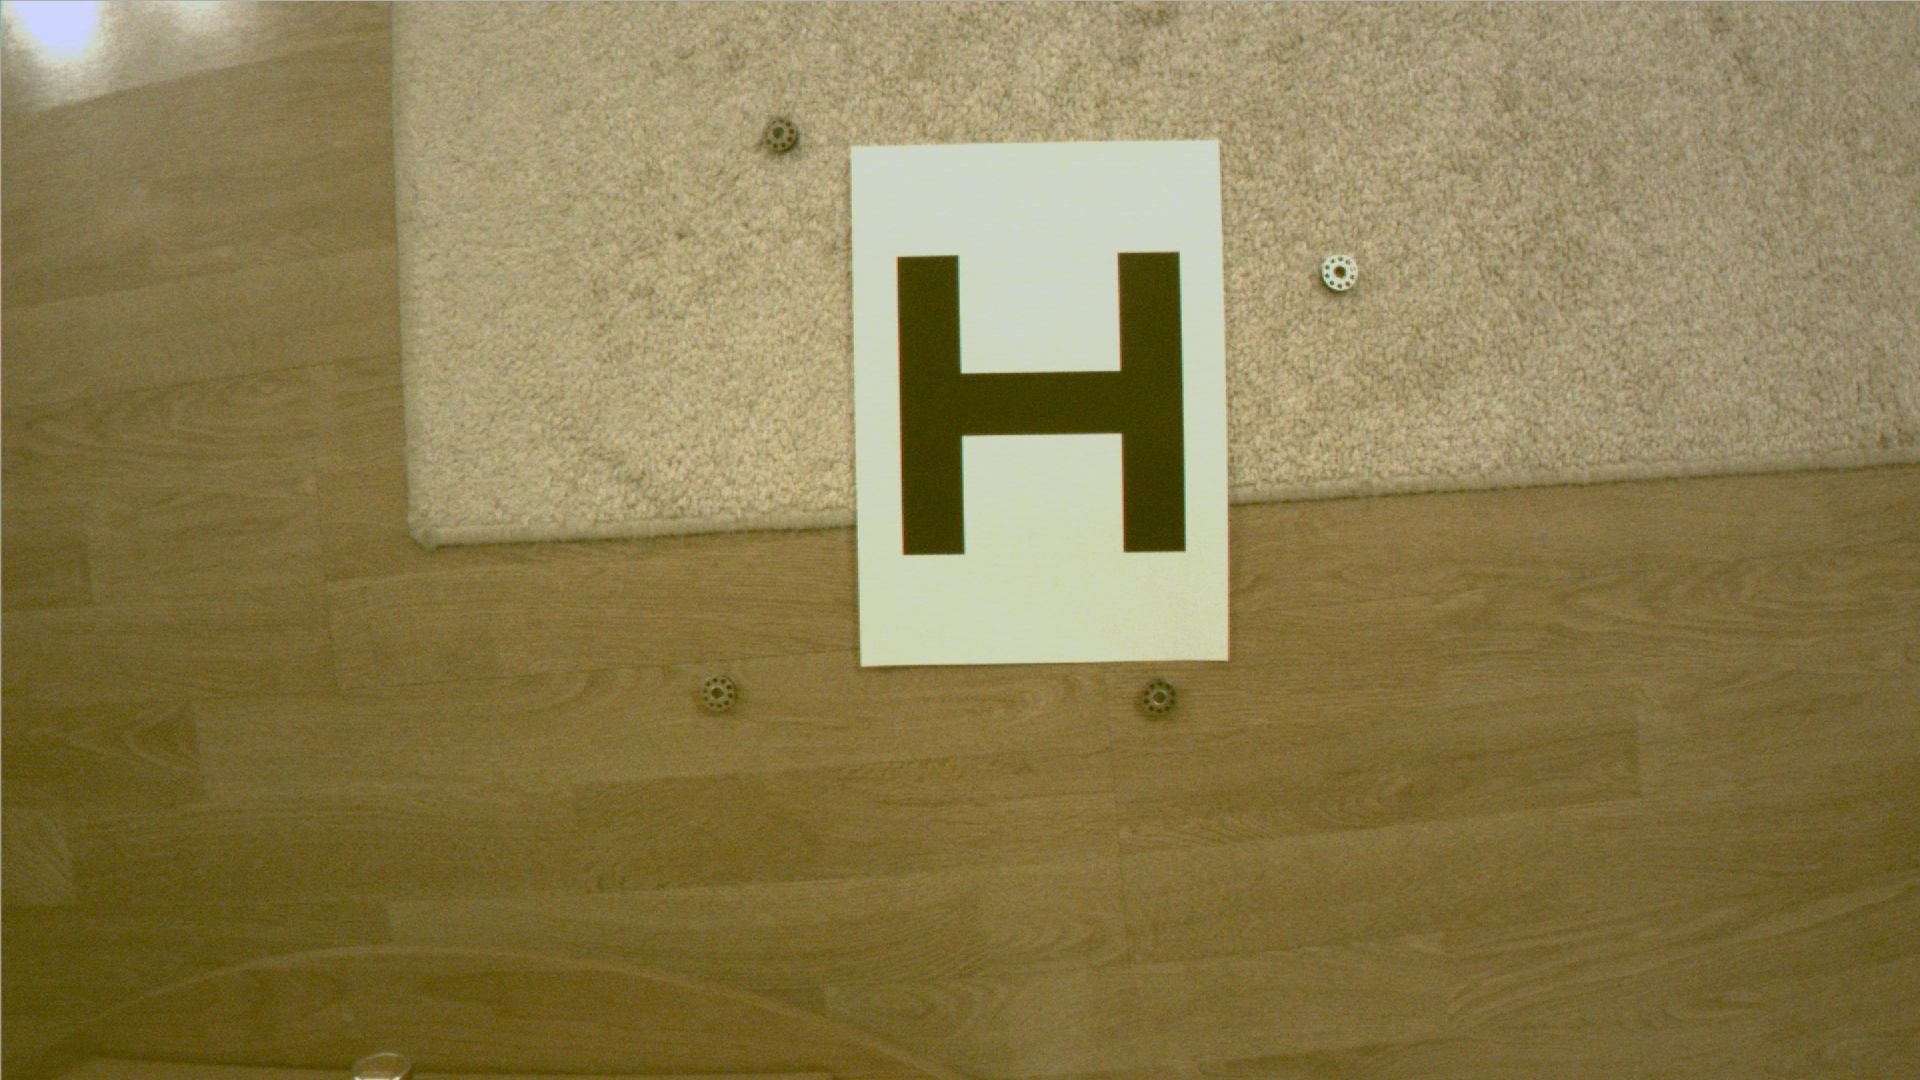
\includegraphics[width=\textwidth]{h.jpg}
		\caption{Obraz wejściowy.}
		\label{fig:h}
	\end{subfigure}
	\begin{subfigure}{0.4\textwidth}
		\centering
		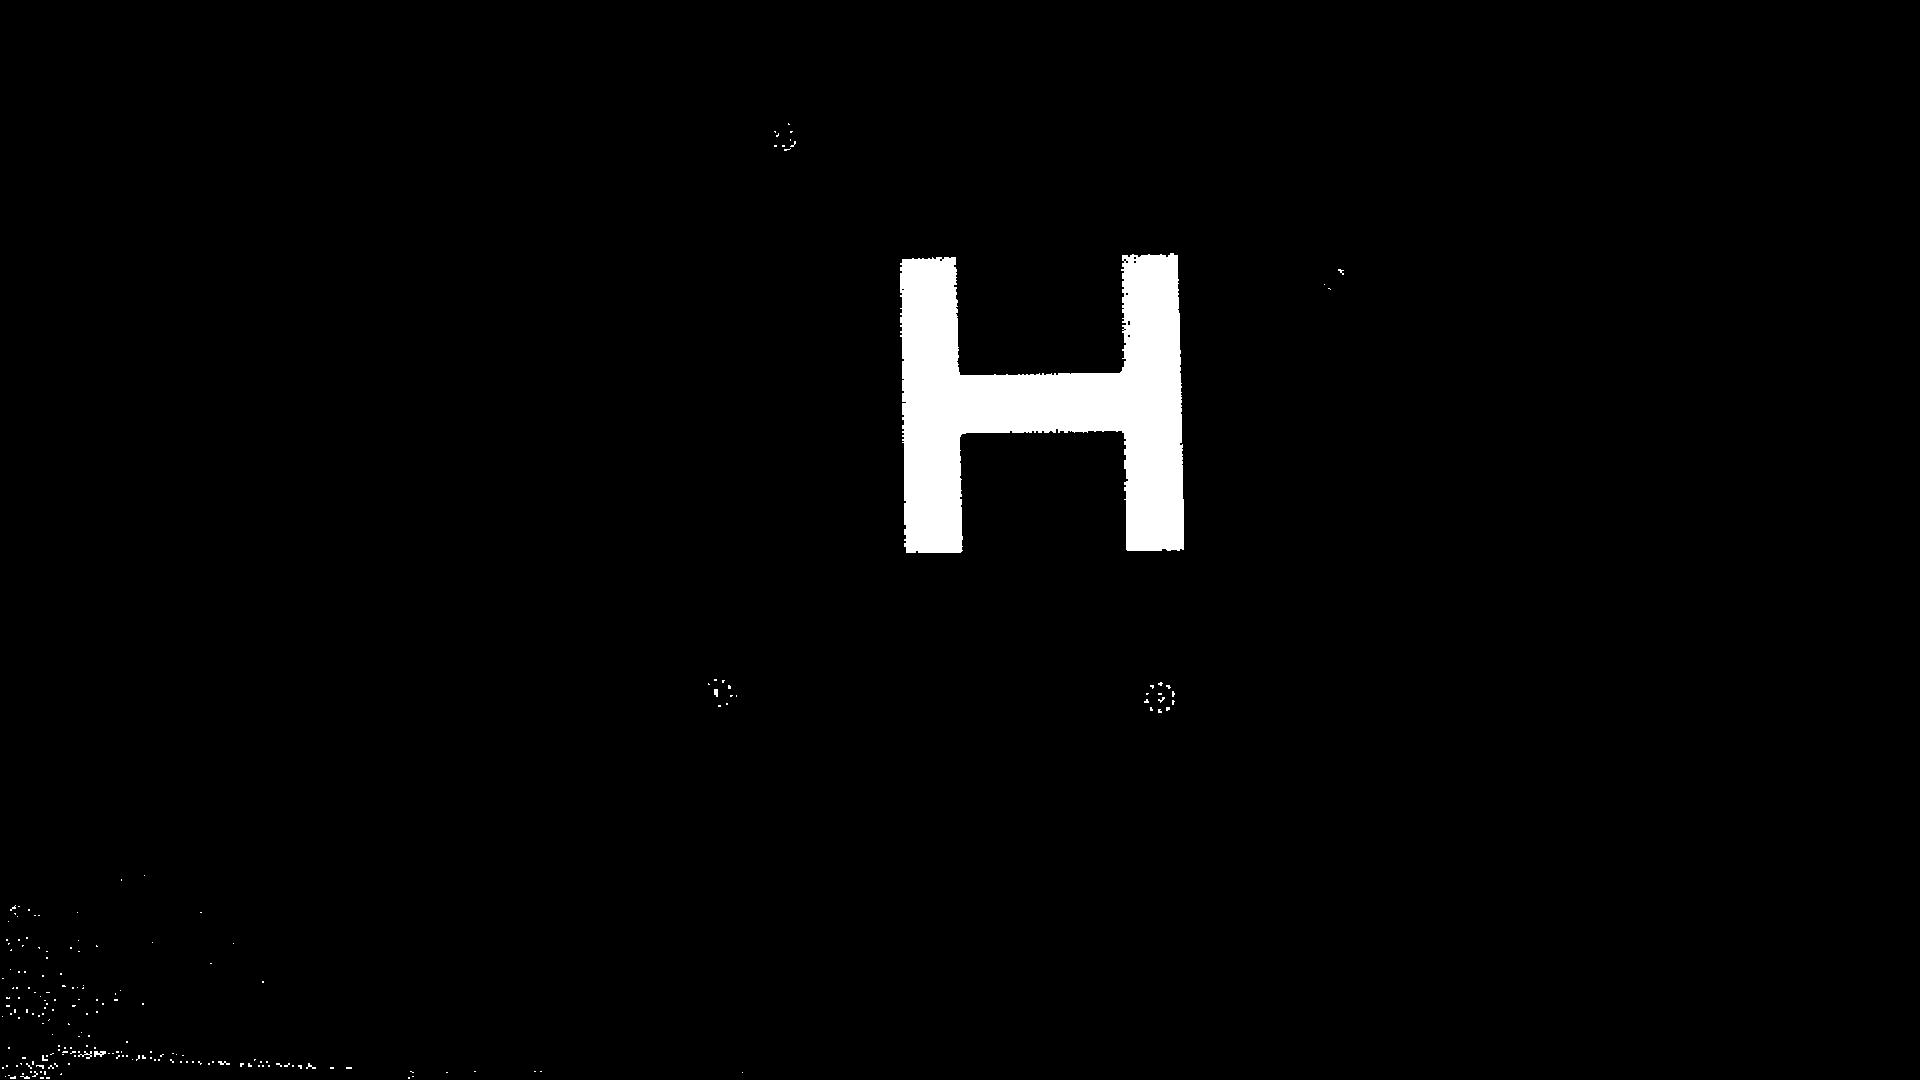
\includegraphics[width=\textwidth]{bin.jpg}
		\caption{Rezultat binaryzacji.}
		\label{fig:bin_1}
	\end{subfigure}\\
	\begin{subfigure}{0.4\textwidth}
		\centering
		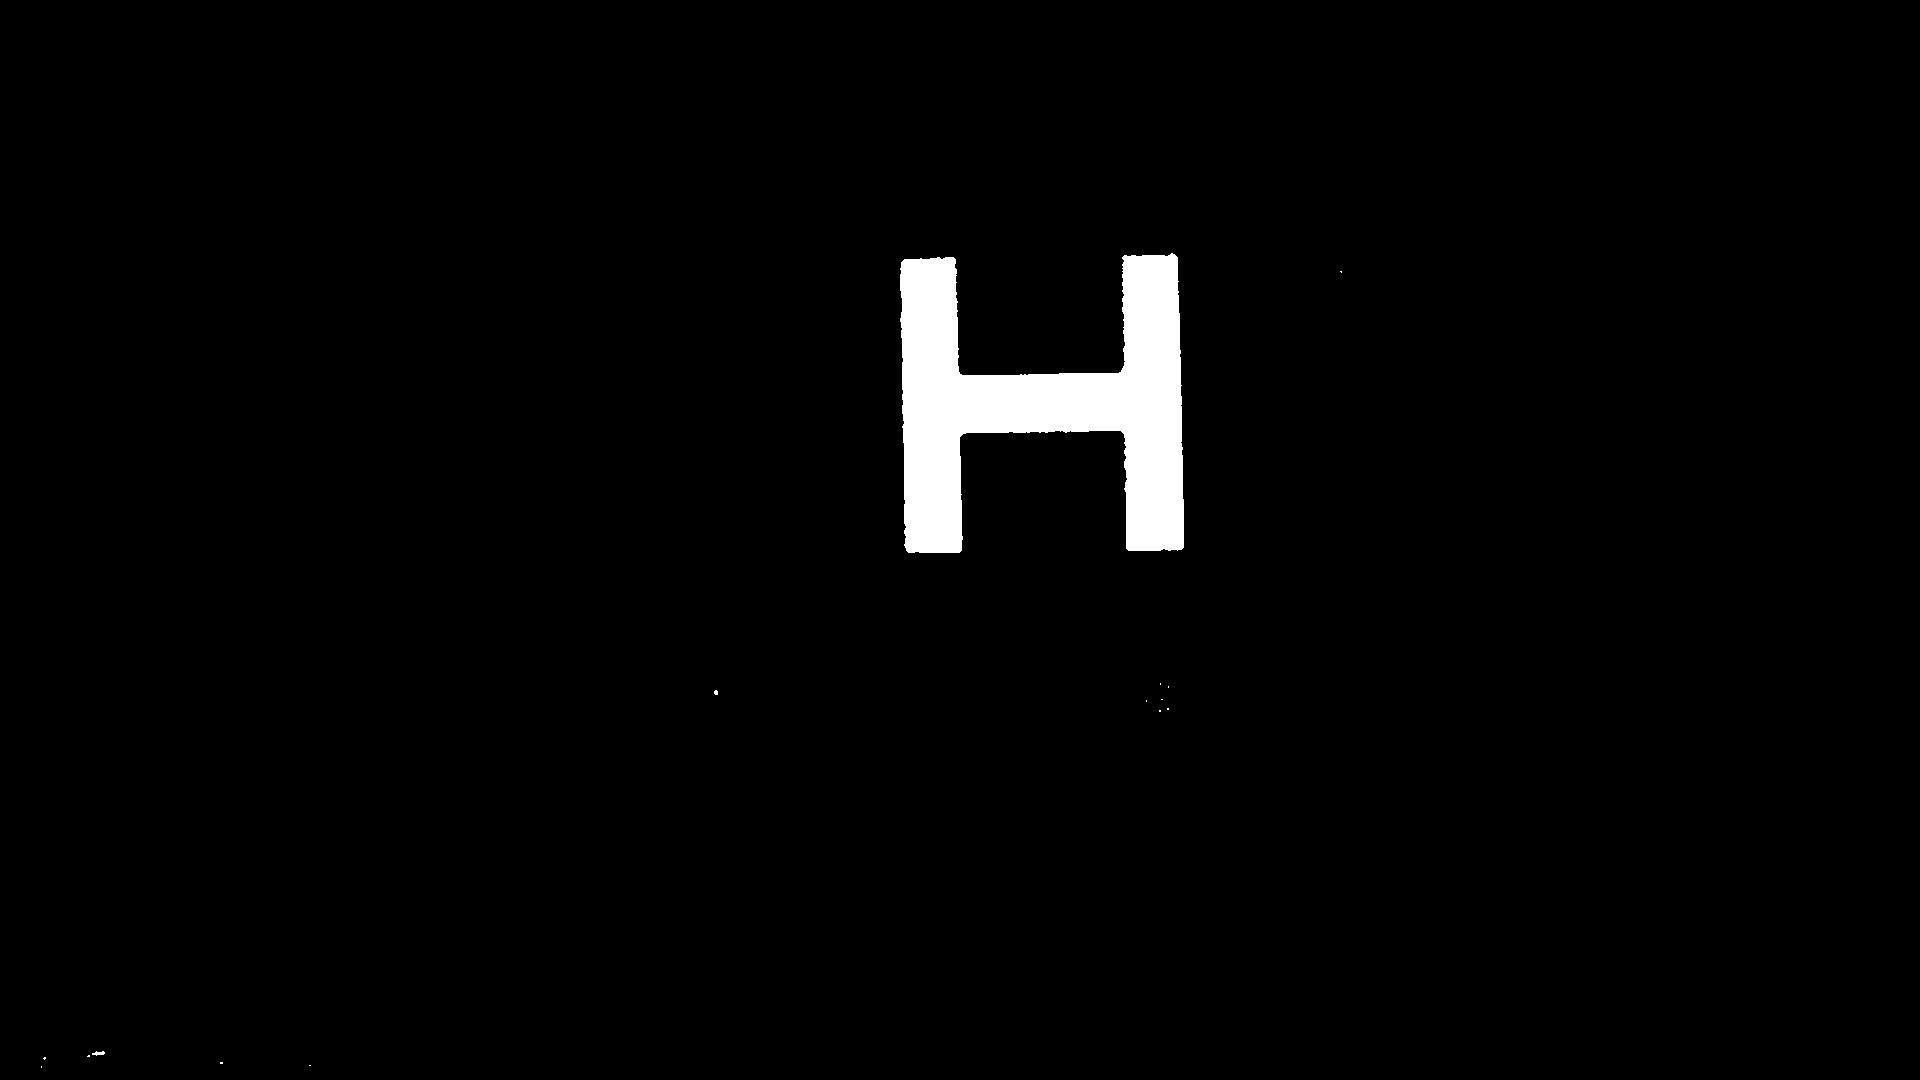
\includegraphics[width=\textwidth]{median.jpg}
		\caption{Obraz po medianie}
		\label{fig:median_1}
	\end{subfigure}
	\begin{subfigure}{0.4\textwidth}
		\centering
		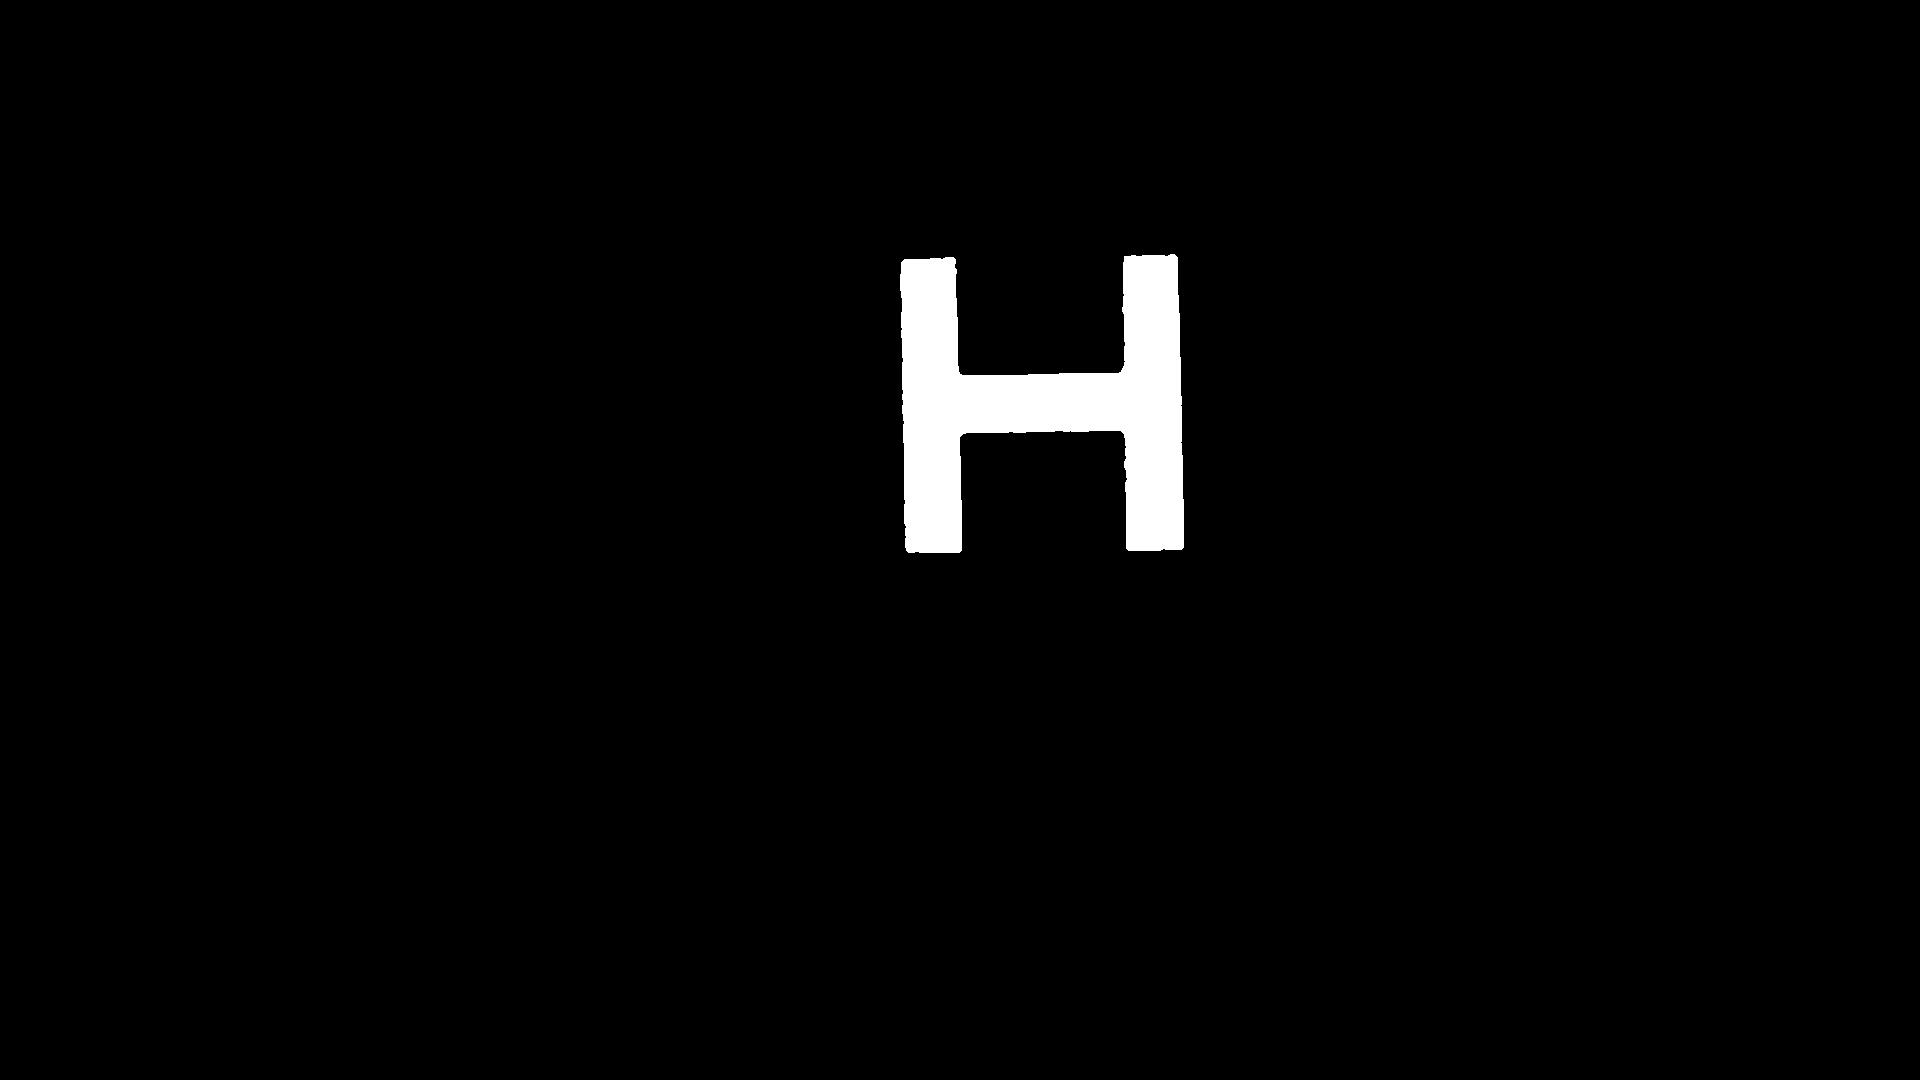
\includegraphics[width=\textwidth]{opened.jpg}
		\caption{Wynik otwarcia}
		\label{fig:opened_1}
	\end{subfigure}
	\caption{Przykładowe rezultaty binaryzacji, mediany i~otwarcia obrazu.}
	\label{fig:operacje}
\end{figure}


\section{Wybór znacznika} 
\label{sec:wybor_znacznika}

Autonomiczne lądowanie drona w~oparciu o~system wizyjny wymaga wyposażenia lądowiska w~marker. 
Jego wygląd musi umożliwiać łatwą detekcję miejsca lądowania. 
Z~powodu wykonywania operacji na~zewnątrz, znacznik powinien również ułatwiać znalezienie go~w~zmiennych warunkach (zachmurzenie, cień).

\subsection{Kształt}
\label{subsec:ksztalt} 
Detekcja kształtów może być realizowana na~różne sposoby. 
Najprostszym jest progowanie współczynników kształtu, do~bardziej zaawansowanych należy wyspecjalizowana deskrypcja cech (SIFT (ang. \textit{Scale-Invariant Feature Transform}), SURF (ang. \textit{Speeded-Up Robust Features}), HOG (ang. \textit{Histogram of Oriented Gradients})) i~użycie klasyfikatorów (kNN (ang. \textit{k-Nearest Neighbours}), SVM (ang. \textit{Support Vector Machine}), sieci neuronowe).
W~implementowanej pierwszej wersji systemu zdecydowano się na~klasyfikację przy użyciu współczynnika kształtu.

Cechami obiektu łatwymi do~wyliczenia w~systemie potokowym są~pole figury i~najmniejszy prostokąt, w~którym figura się mieści (prostokąt otaczający). 
Postanowiono zatem wykorzystać współczynnik kształtu przedstawiony we~wzorze \ref{eq:wspolczynnik}.\\
\begin{equation} \label{eq:wspolczynnik}
W=\frac{P_p}{P_o}
\end{equation}
Gdzie:
\begin{eqwhere}[2cm]
	\item[$W$] współczynnik kształtu,
	\item[$P_p$] pole prostokąta otaczającego,
	\item[$P_o$] pole obiektu.
\end{eqwhere}
Aby~taki współczynnik umożliwiał detekcję należało dobrać odpowiedni kształt znacznika. 
Zdecydowano się na~krzyż, gdyż przy każdej jego orientacji pole prostokąta jest znacznie większe od~pola obiektu. 
Dodatkowo, zastosowanie krzyża wydłużonego może dostarczyć informacji o~orientacji znacznika.
\subsection{Kolor}
\label{subsec:kolor}

Kolor znacznika powinien umożliwiać jego łatwą segmentację. 
Z~tego powodu pożądane jest silne skontrastowanie figury i~tła. 
Najbardziej naturalnym rozwiązaniem jest rozważenie kontrastu w~przestrzeni barw RGB, gdyż taki sygnał jest dostarczany przez kamerę.

\begin{figure}[h]
	\centering
	\begin{subfigure}{0.4\textwidth}
		\centering
		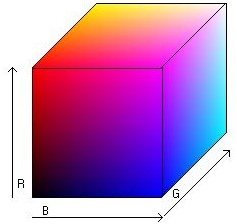
\includegraphics[width=0.5\textwidth]{szescian_rgb.jpg}
		\caption{Przedstawienie przestrzeni barw RGB w~postaci sześcianu \cite{obrazek_rgb}}
		\label{fig:szescian_rgb}
	\end{subfigure}%
	\begin{subfigure}{0.4\textwidth}
		\centering
		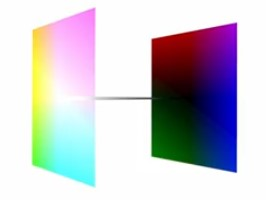
\includegraphics[width=0.5\textwidth]{szescian_ycbcr.jpg}
		\caption{Przekroje sześcianu przestrzeni YCbCr \cite{obrazek_ycbcr}}
		\label{fig:szescian_ycbcr}
	\end{subfigure}%
	\caption{Modele przestrzeni RGB i YCbCr}
	\label{fig:modele_przestrzeni}
\end{figure}

W~przestrzeni RGB każdy piksel opisywany jest przez trzy składowe: czerwoną, zieloną i~niebieską. 
Możliwe jest przedstawienie tego systemu w~formie sześcianu (rys. \ref{fig:szescian_rgb}). 
Można wyznaczyć przekątną łączącą punkty, dla których wszystkie współrzędne są~identyczne. 
Rozciąga się ona od~koloru czarnego w~początku układu współrzędnych, do~białego dla~maksymalnych wartości składowych, przechodząc przez różne stopnie szarości. 
Wykorzystanie dużej odległości między kolorami i~użycie czarno-białego znacznika wydaje się zatem najprostszym pomysłem.

W~pierwszym kroku do testów przygotowano czarny znacznik na~białym tle. 
Kamerą PCAM 5C wykonano trzy zdjęcia przy różnym poziomie oświetlenia (rys. \ref{fig:osw1}, \ref{fig:osw2}, \ref{fig:osw3}). 
Wykonanie takich zdjęć było możliwe po implementacji akwizycji ramek na~kartę~SD  (podrozdział \ref{sec:image_sd}). 
Po~przejściu na~obraz w~skali szarości, posługując się narzędziem \textit{roipoly} w~programie Matlab, obliczono histogramy obszaru znacznika (rys. \ref{fig:bw_hist1}, \ref{fig:bw_hist2}, \ref{fig:bw_hist3}).\\
\begin{figure}
	\centering
	\begin{subfigure}{0.4\textwidth}
		\centering
		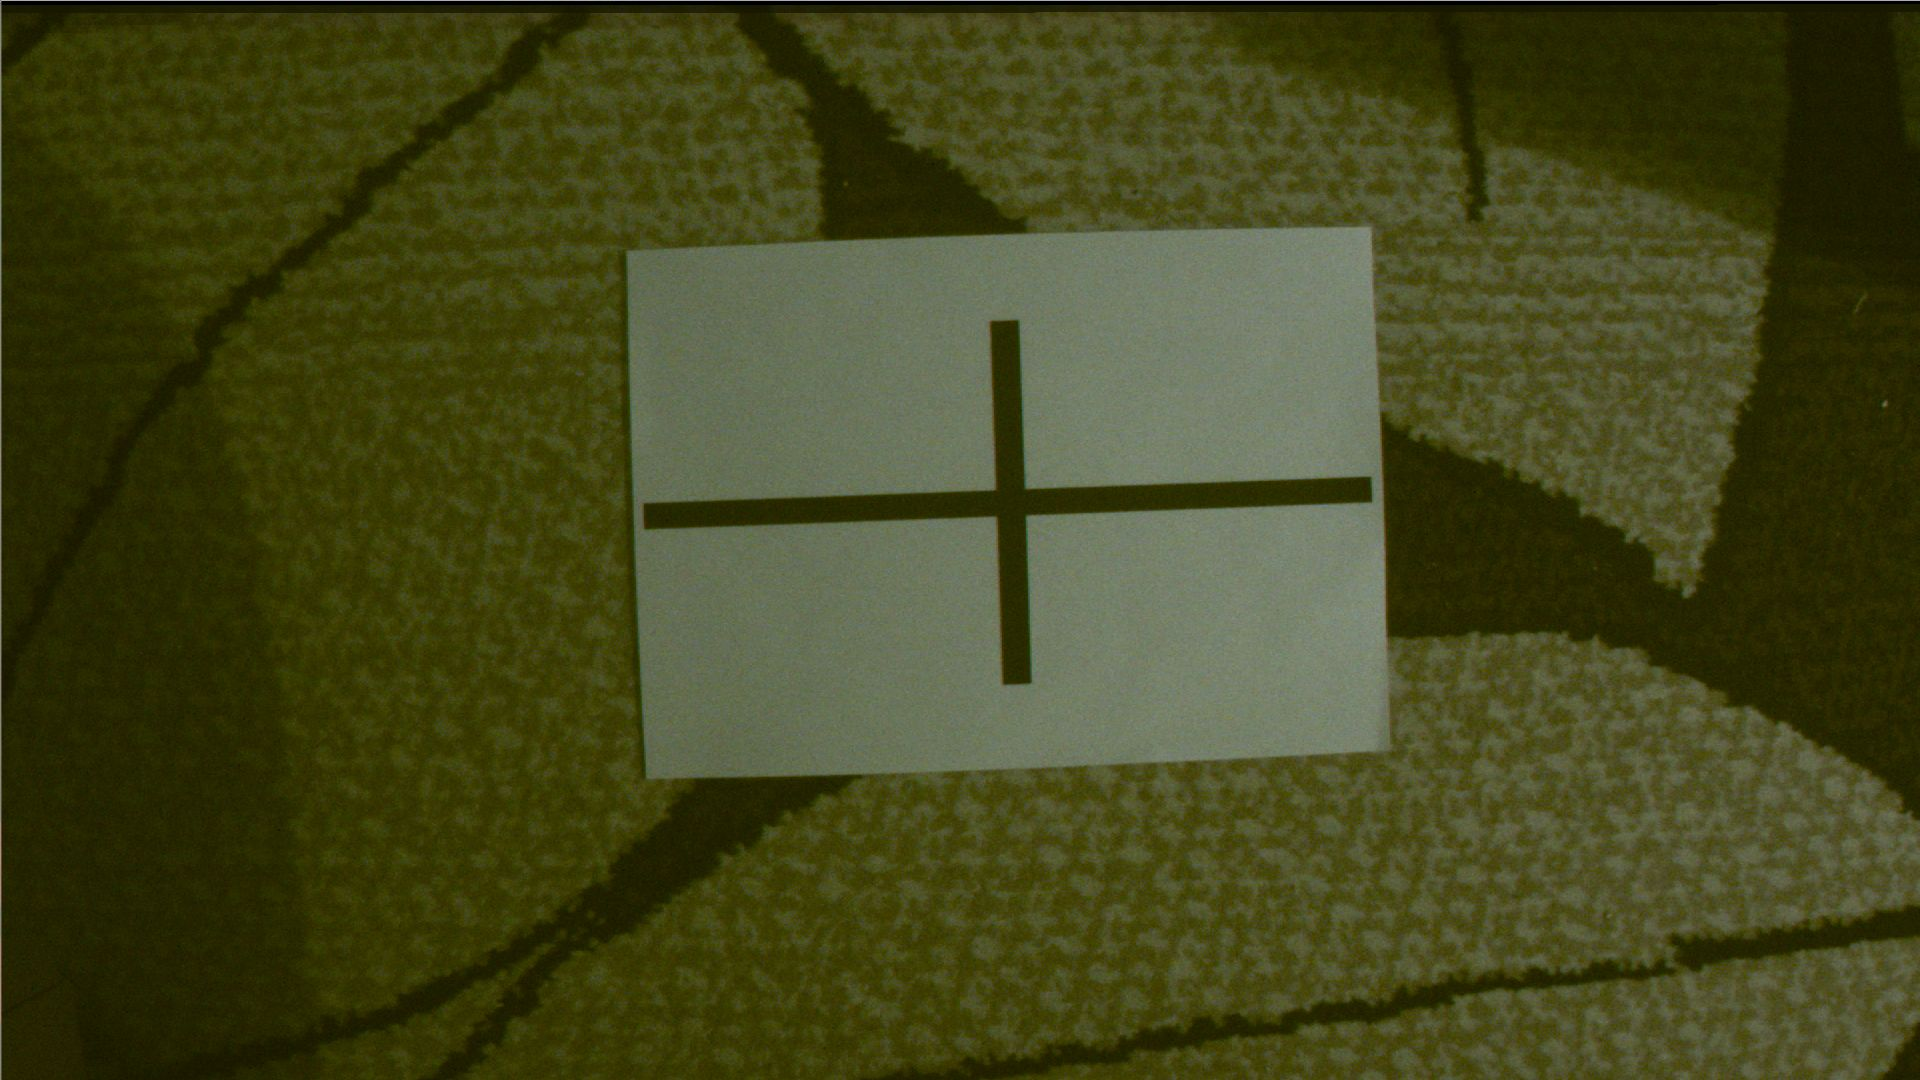
\includegraphics[width=0.98\textwidth]{rgb_ciemny.jpg}
		\caption{}
		\label{fig:osw1}
	\end{subfigure}%
	\begin{subfigure}{0.55\textwidth}
		\centering
		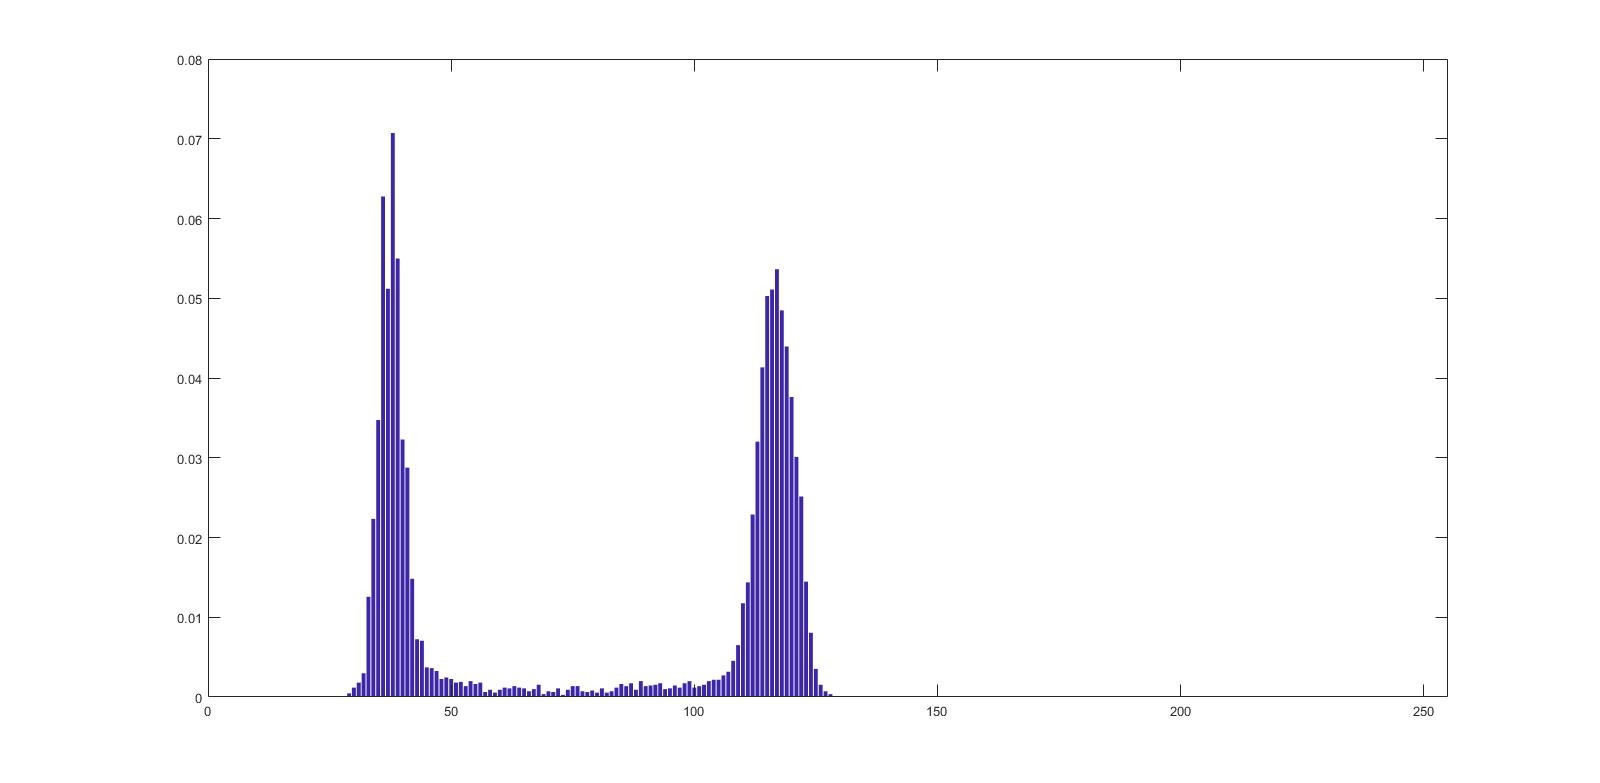
\includegraphics[width=0.98\textwidth]{bw_hist1.jpg}
		\caption{}
		\label{fig:bw_hist1}
	\end{subfigure}\\
	\begin{subfigure}{0.4\textwidth}
		\centering
		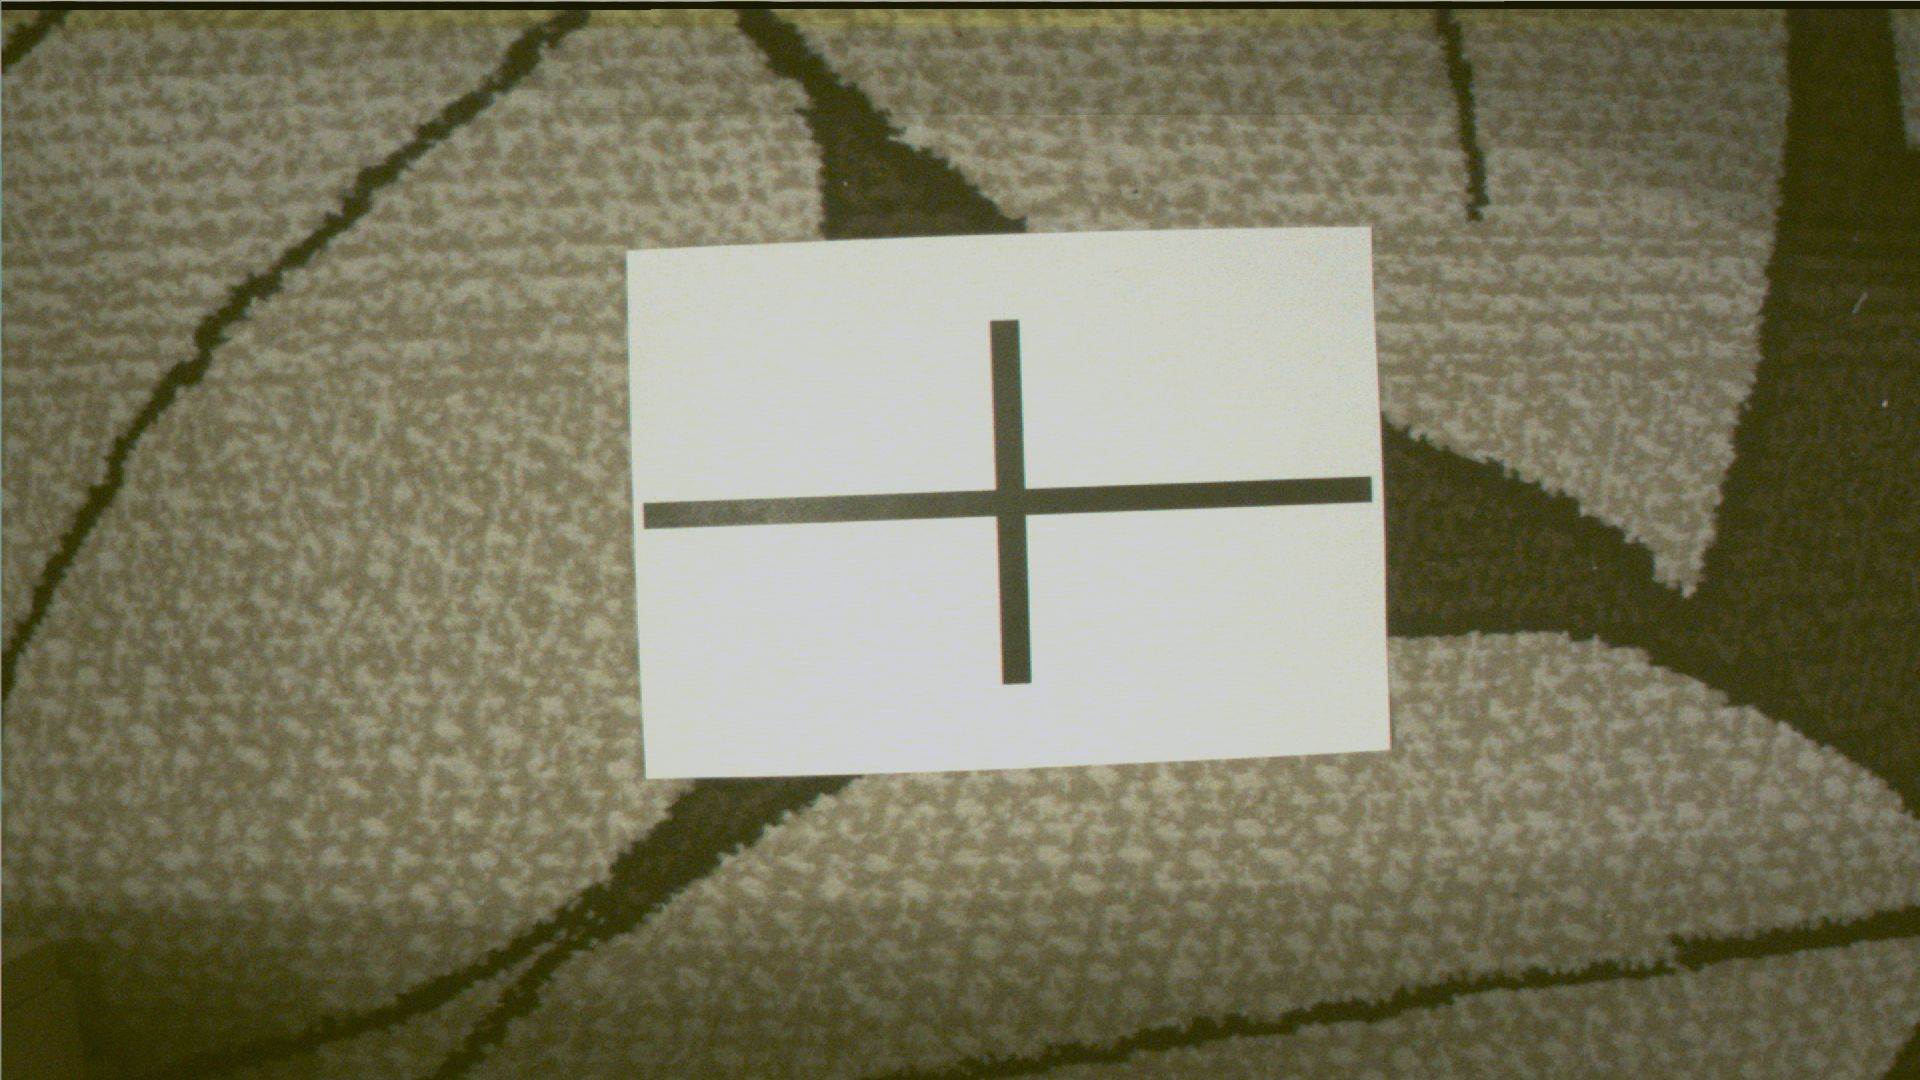
\includegraphics[width=0.98\textwidth]{rgb_sredni.jpg}
		\caption{}
		\label{fig:osw2}
	\end{subfigure}
	\begin{subfigure}{0.55\textwidth}
		\centering
		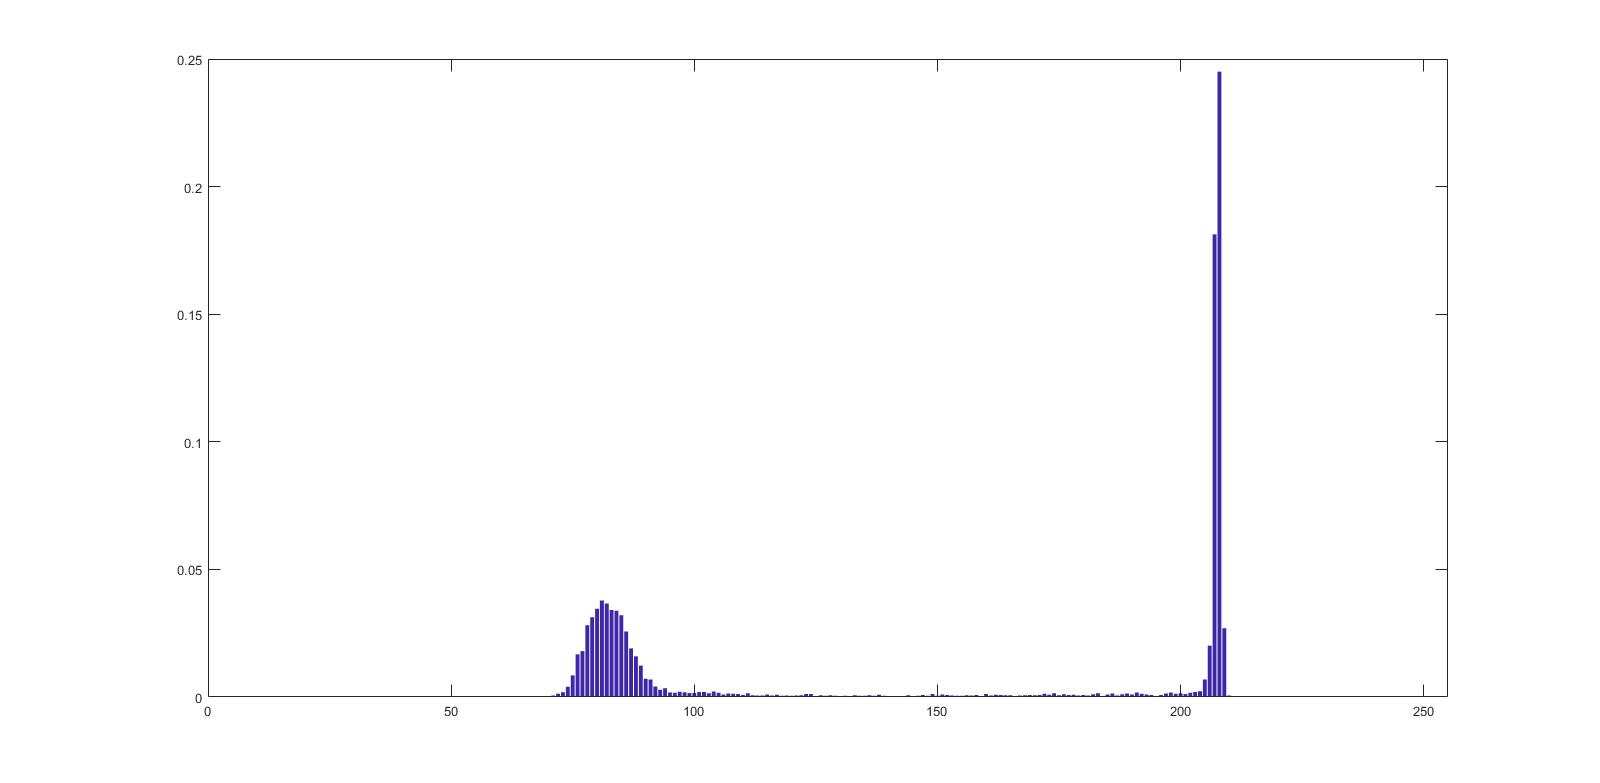
\includegraphics[width=0.98\textwidth]{bw_hist2.jpg}
		\caption{}
		\label{fig:bw_hist2}
	\end{subfigure}\\
	\begin{subfigure}{0.4\textwidth}
		\centering
		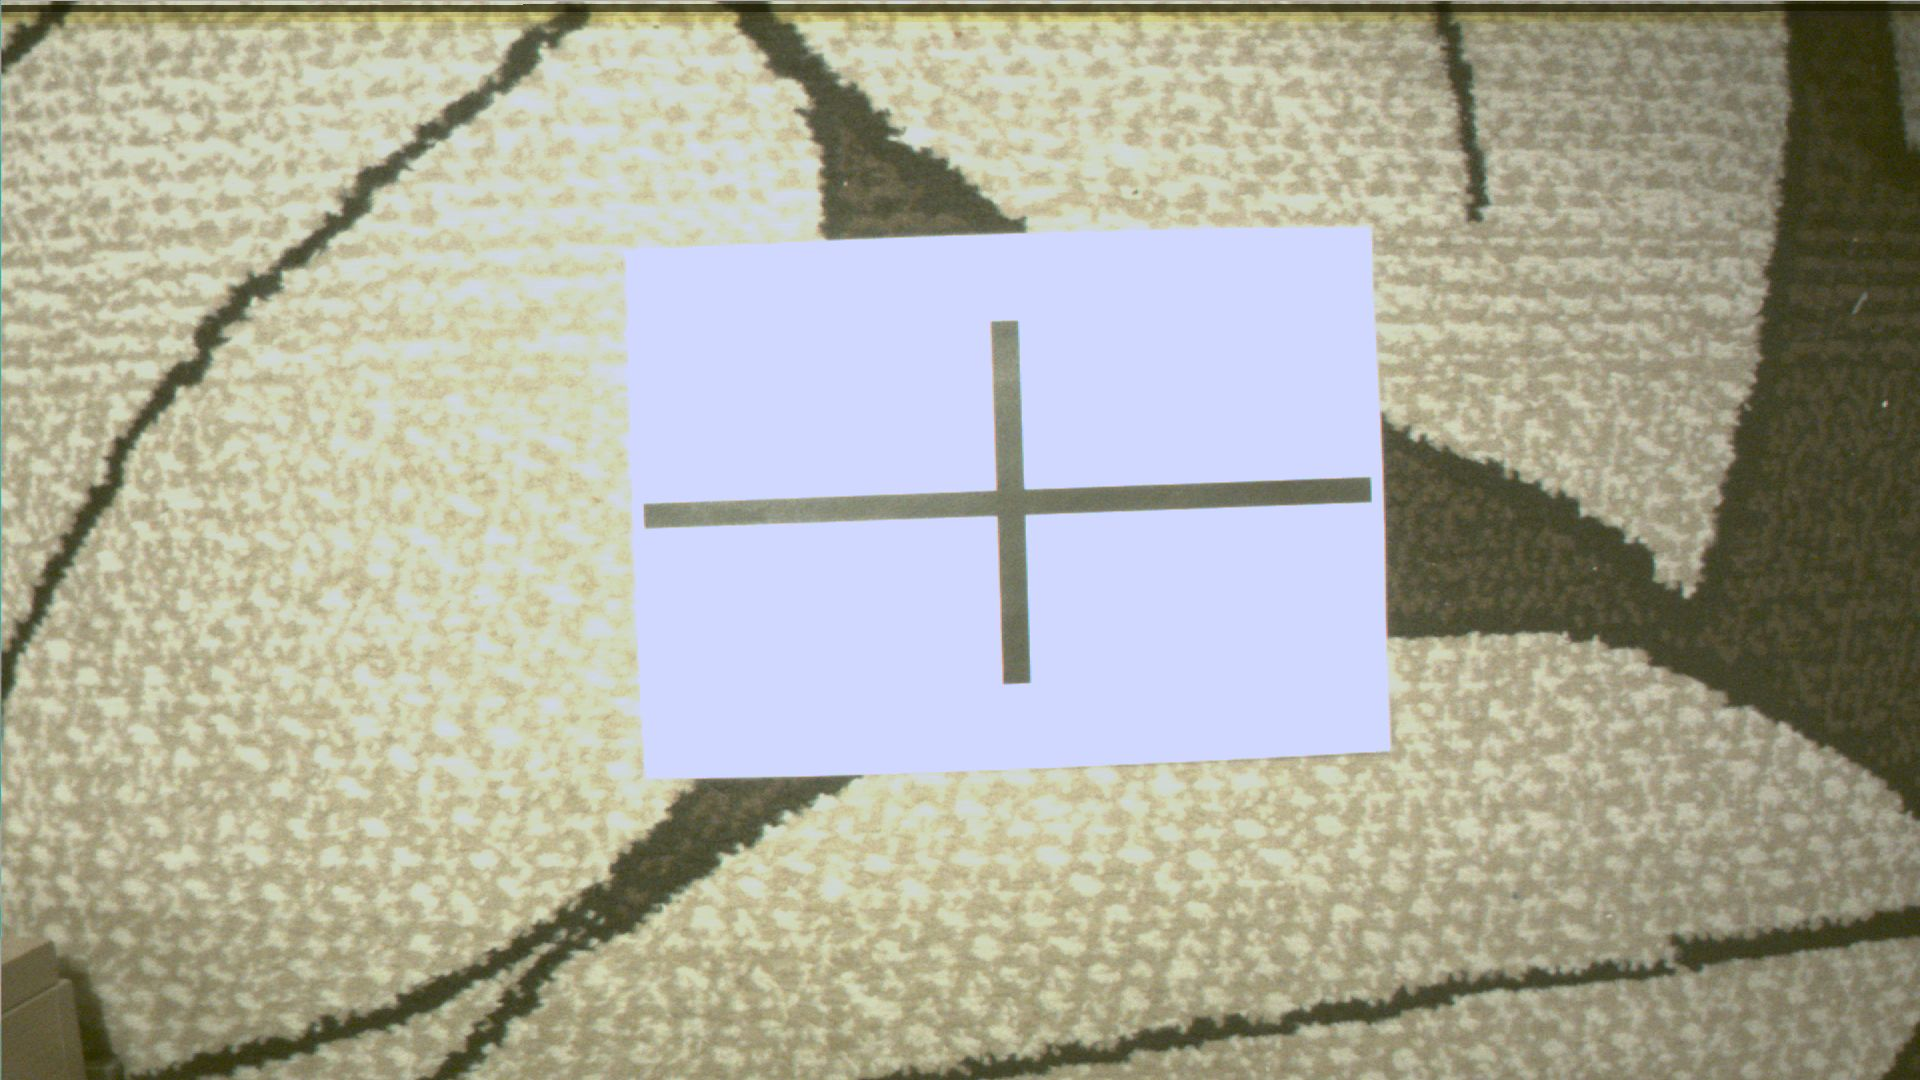
\includegraphics[width=0.98\textwidth]{rgb_jasny.jpg}
		\caption{}
		\label{fig:osw3}
	\end{subfigure}
	\begin{subfigure}{0.55\textwidth}
		\centering
		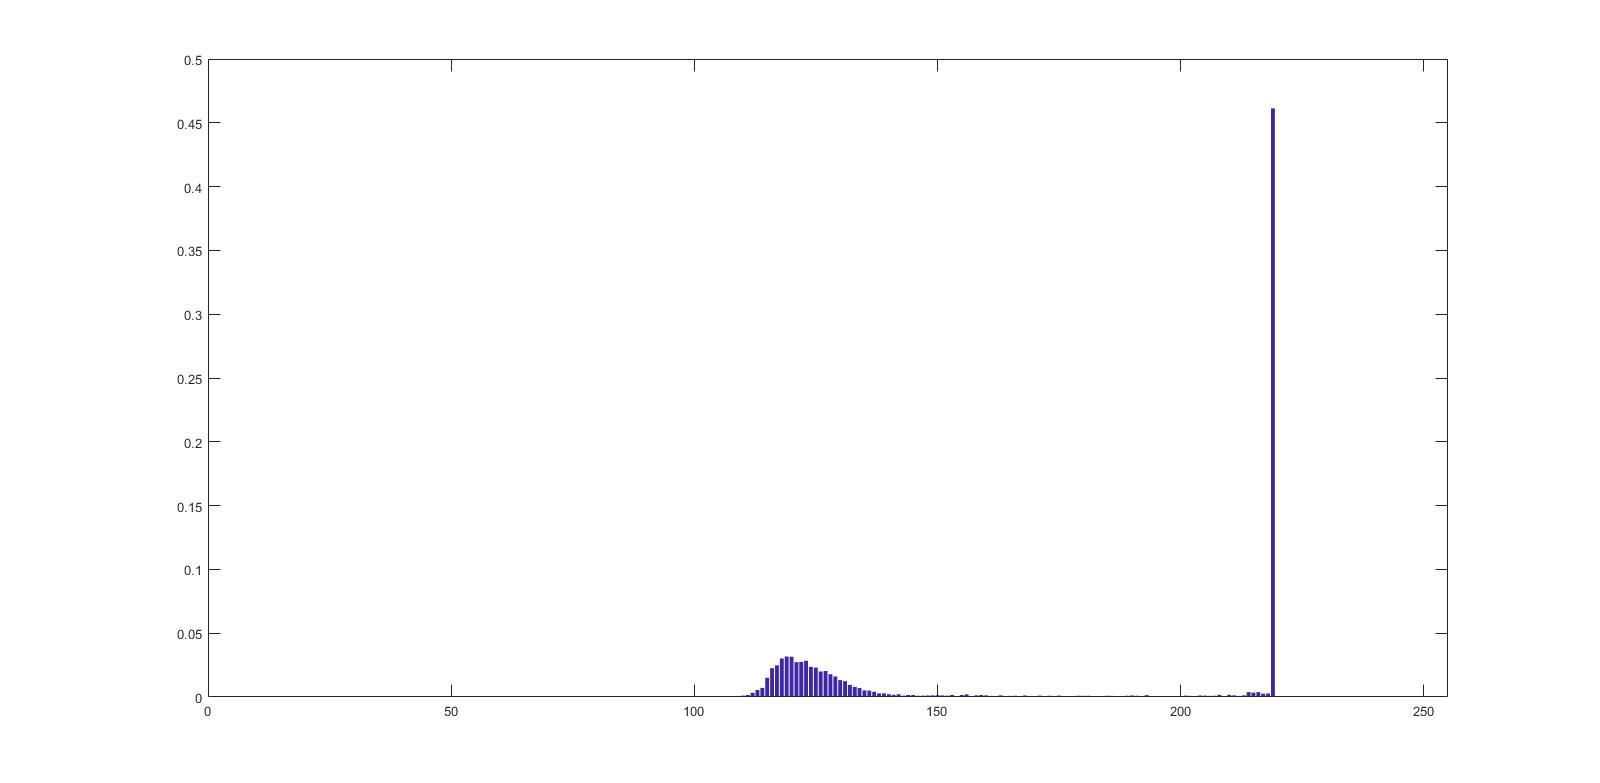
\includegraphics[width=0.98\textwidth]{bw_hist3.jpg}
		\caption{}
		\label{fig:bw_hist3}
	\end{subfigure}
	\caption{Zdjęcia pierwszej wersji znacznika wraz z~histogramami obszaru znacznika}
	\label{fig:zdjecia_wejsciowe}
\end{figure}

Analiza histogramów wskazuje na~silne uzależnienie położenia maksimów odpowiadających tłu i~znacznikowi od~oświetlenia.  
Dla kolejnych obrazów, wartości progów binaryzacji mogłyby zawierać się w~zakresach: 50-100, 100-200, 150-210. Poziom białego tła dla obrazka najsłabiej oświetlonego jest mniejszy niż wartość czarnego koloru znacznika najlepiej oświetlonego. 
W~takiej sytuacji niemożliwy jest dobór stałego progu umożliwiającego skuteczną binaryzację.

Z~tego powodu zdecydowano się na~powtórzenie eksperymentu w~przestrzeni YCbCr. 
Tak jak opisano w~rozdziale \ref{sec:opis_operacji}, piksel w~tej przestrzeni opisuje współrzędna luminancji i~dwie składowe chrominacji. 
Podobnie jak w~przypadku RGB, przestrzeń YCbCr również da~się przedstawić w~postaci sześcianu. 
Tym razem skala szarości przebiega przez środek płaszczyzn Cb-Cr i~za zmianę poziomu szarości odpowiada współrzędna luminancji (rys. \ref{fig:szescian_ycbcr}). 
Dla~każdej wartości piksela informacja o~jasności oddzielona jest od~barwy.

Kolor znacznika określono jako czerwony, natomiast tło niebieskie, gdyż te~barwy znajdują się na~przeciwnych stronach płaszczyzny Cr-Cb. 
Zdjęcia wykonano przy takich samych poziomach oświetlenia jak poprzednio. 
Histogramy kolejnych obrazów przedstawiono na~rysunku \ref{fig:ycbcr_hist1}, \ref{fig:ycbcr_hist2}, \ref{fig:ycbcr_hist3}. 
\begin{figure}
	\centering
	\begin{subfigure}{0.45\textwidth}
		\centering
		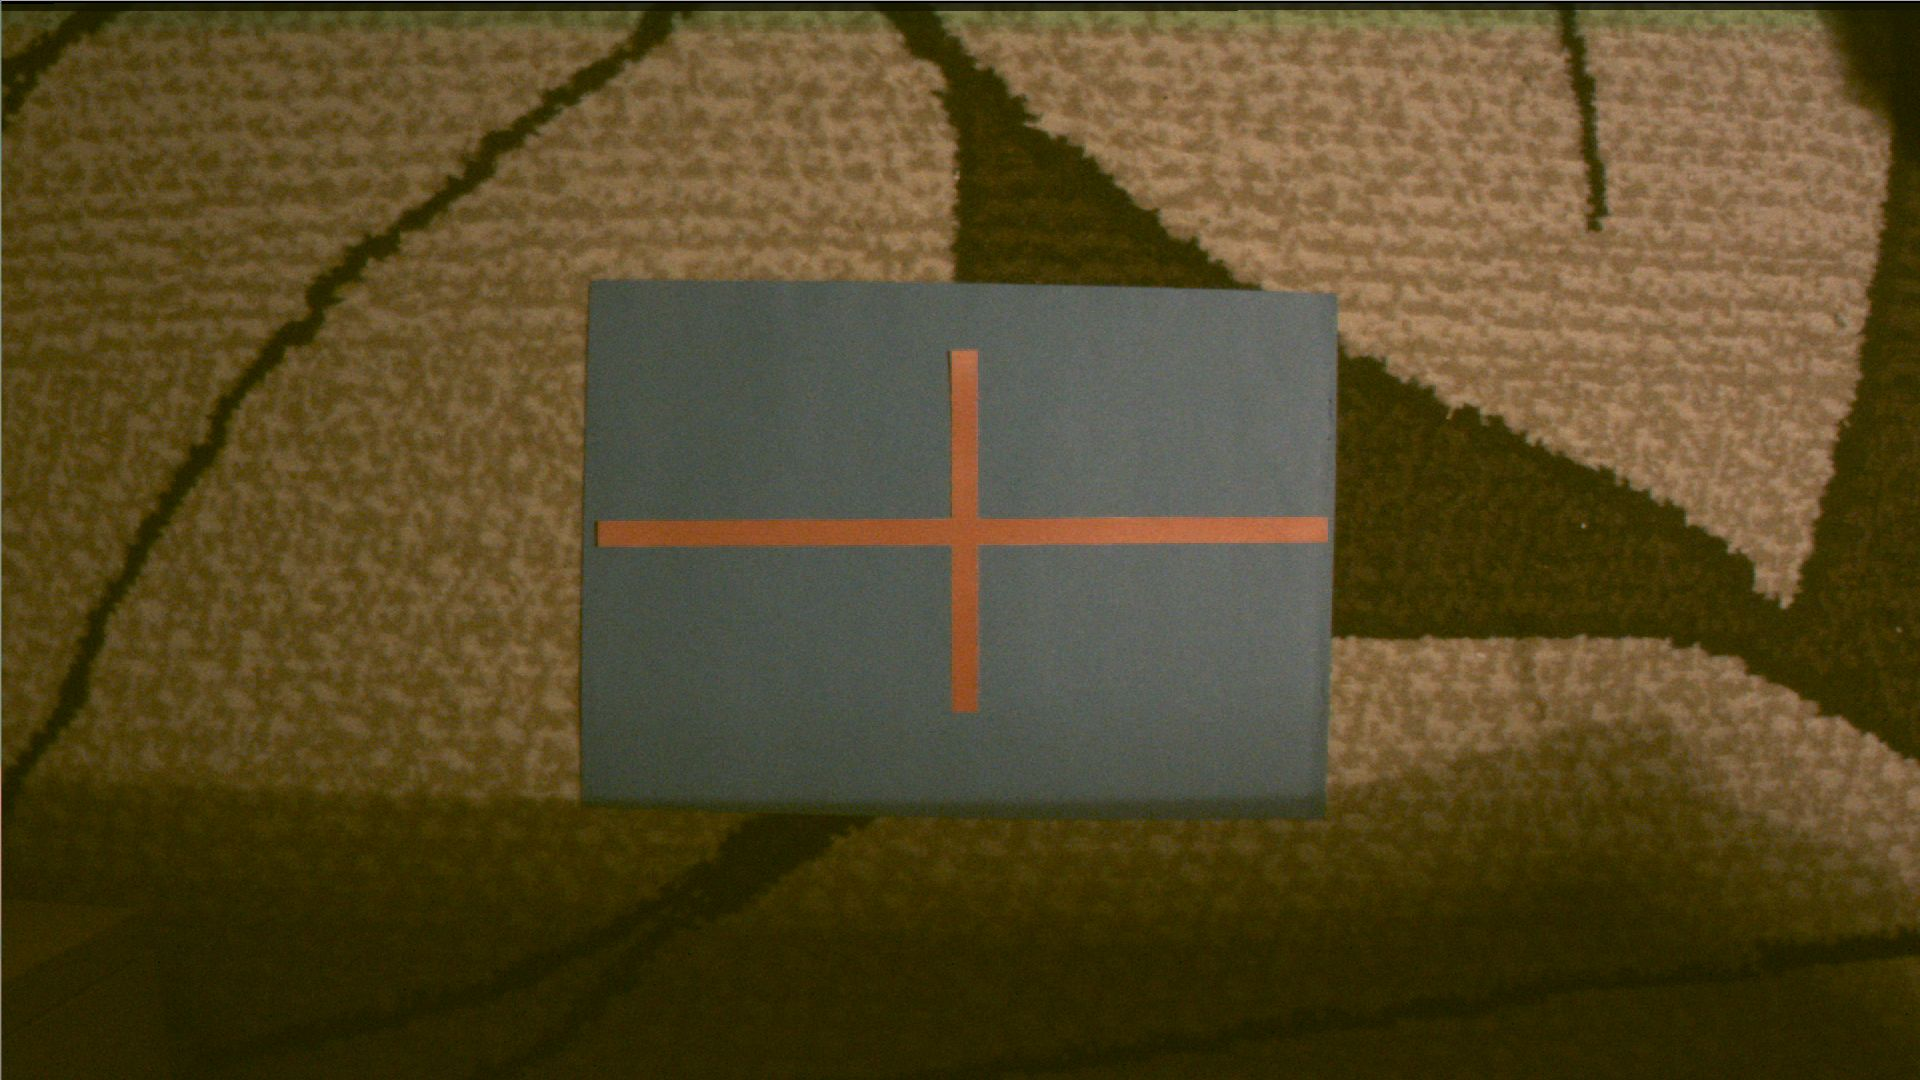
\includegraphics[width=0.9\textwidth]{ycbcr_ciemny.jpg}
		\caption{}
		\label{fig:ycbcr_1}
	\end{subfigure}
	\begin{subfigure}{0.45\textwidth}
		\centering
		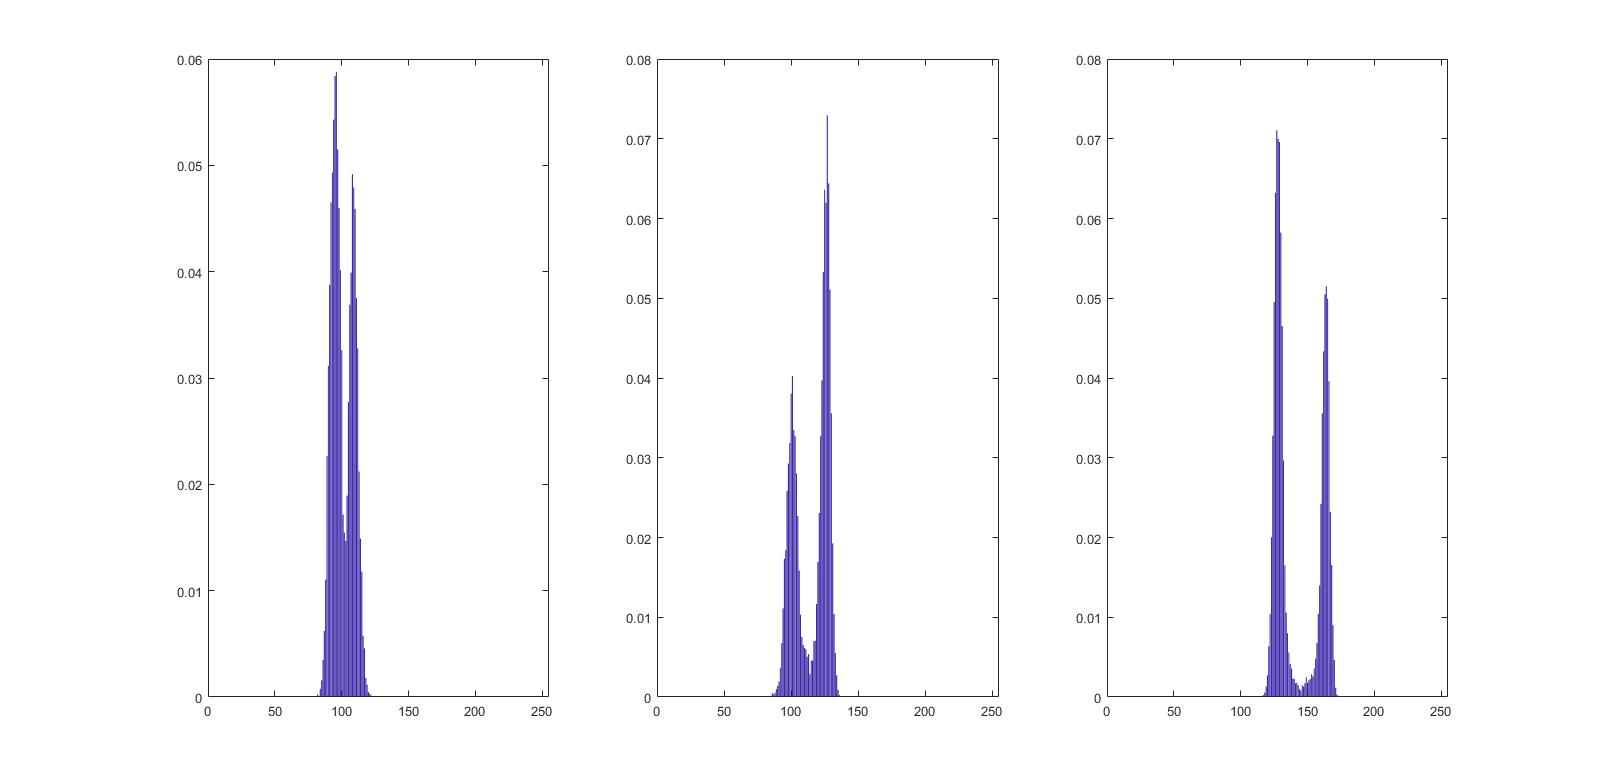
\includegraphics[width=0.9\textwidth]{ycbcr_hist1.jpg}
		\caption{}
		\label{fig:ycbcr_hist1}
	\end{subfigure}\\
	\begin{subfigure}{0.45\textwidth}
		\centering
		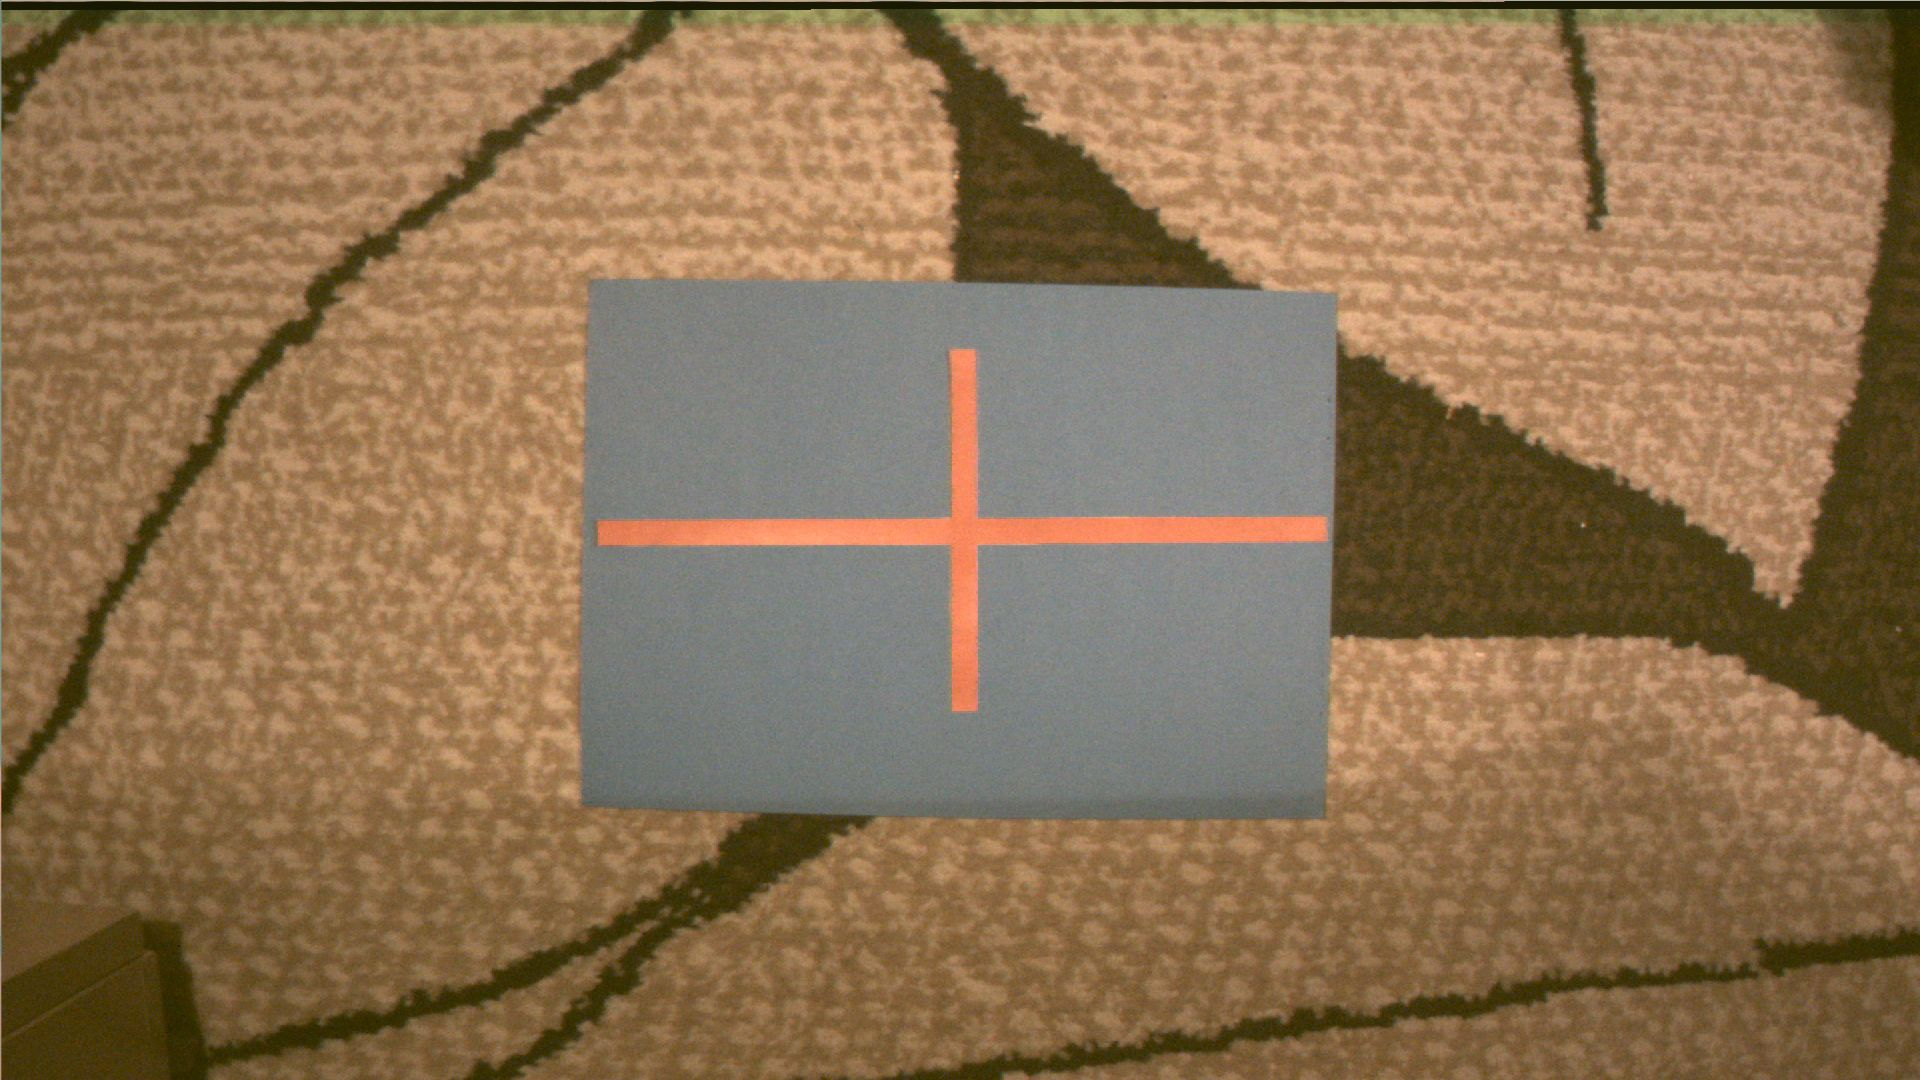
\includegraphics[width=0.9\textwidth]{ycbcr_sredni.jpg}
		\caption{}
		\label{fig:ycbcr_2}
	\end{subfigure}
	\begin{subfigure}{0.45\textwidth}
		\centering
		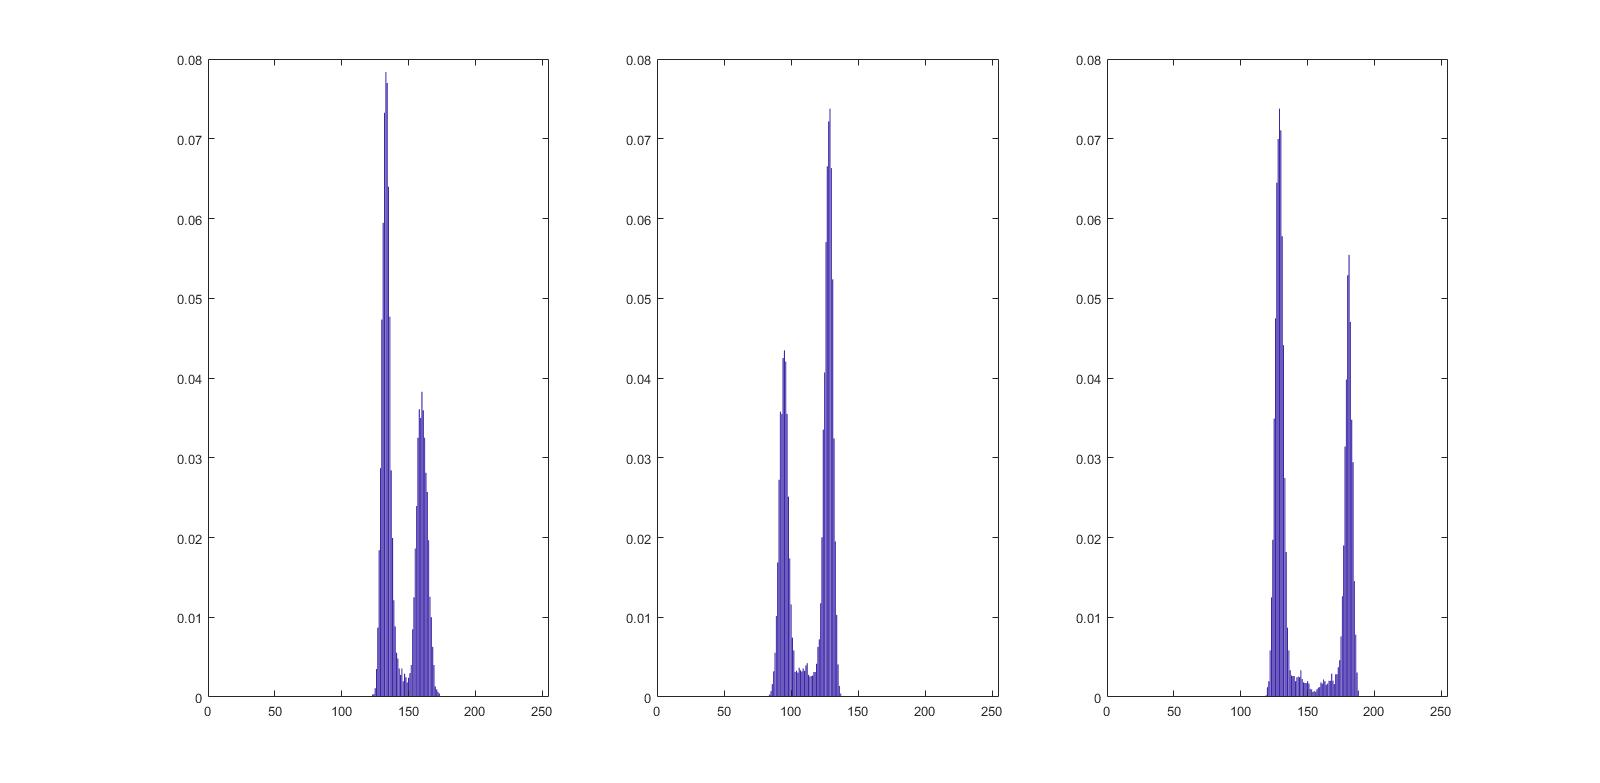
\includegraphics[width=0.9\textwidth]{ycbcr_hist2.jpg}
		\caption{}
		\label{fig:ycbcr_hist2}
	\end{subfigure}\\
	\begin{subfigure}{0.45\textwidth}
		\centering
		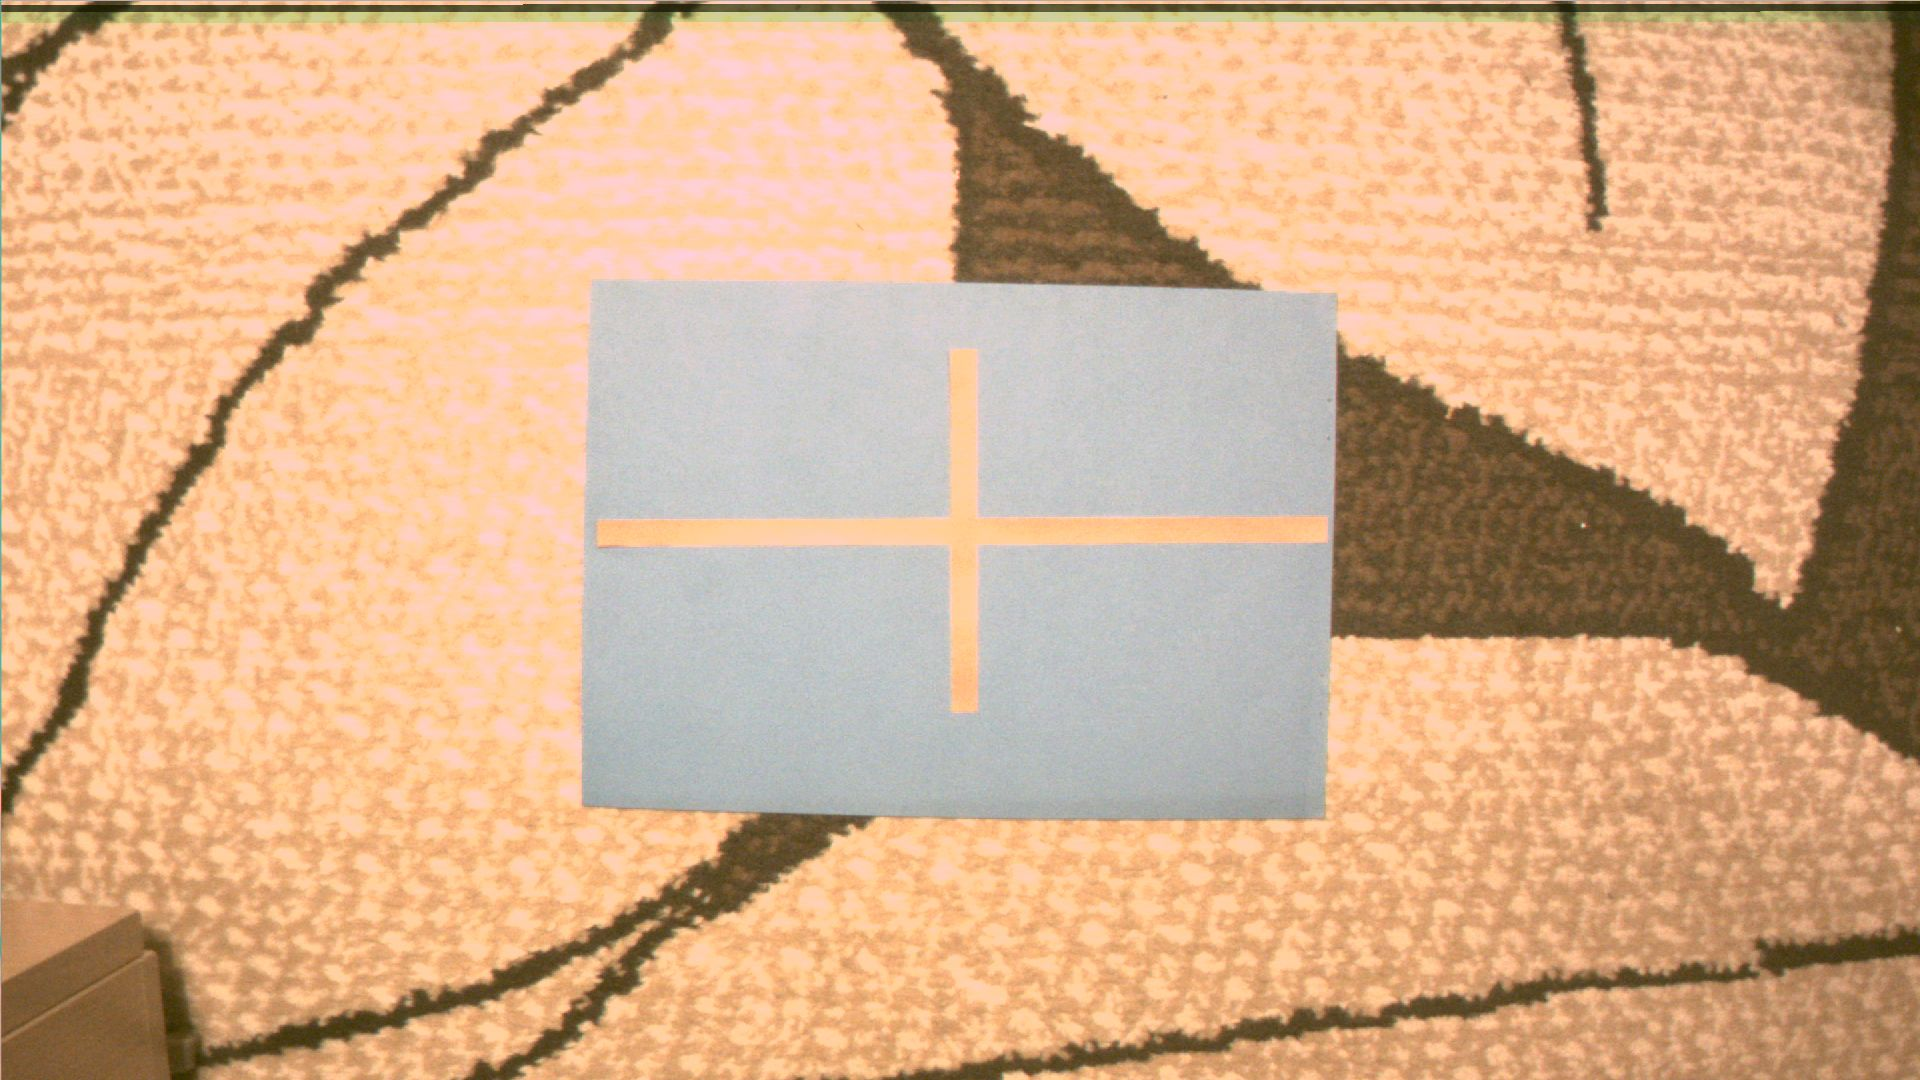
\includegraphics[width=0.9\textwidth]{ycbcr_jasny.jpg}
		\caption{}
		\label{fig:ycbcr_3}
	\end{subfigure}
	\begin{subfigure}{0.45\textwidth}
		\centering
		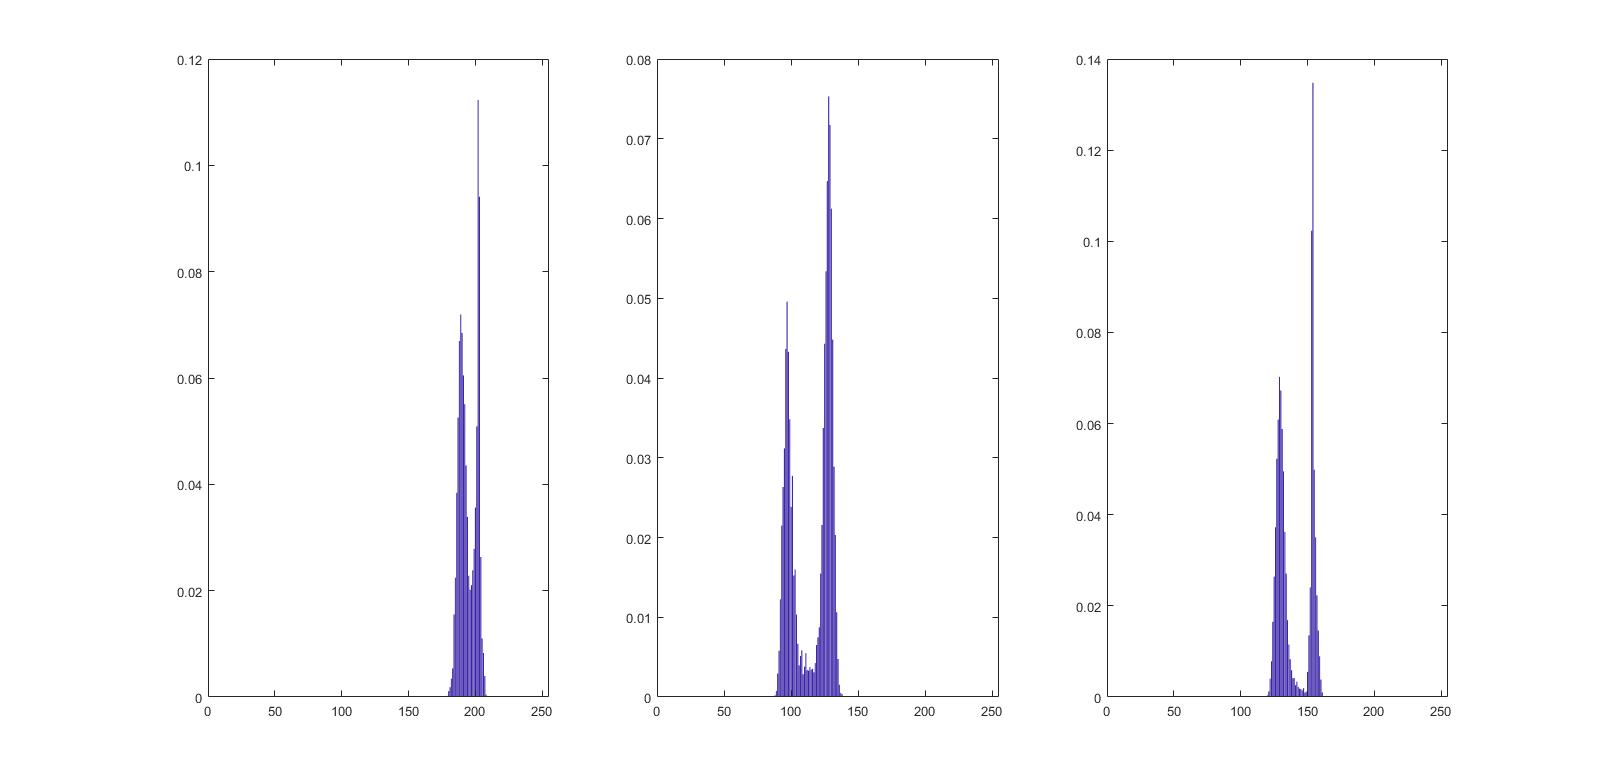
\includegraphics[width=0.9\textwidth]{ycbcr_hist3.jpg}
		\caption{}
		\label{fig:ycbcr_hist3}
	\end{subfigure}
	\caption{Obrazy i histogramy obszarów znacznika w~przestrzeni YCbCr.}
	\label{fig:histogramy_ycbcr}
\end{figure}

Zgodnie z~oczekiwaniami, zmiana poziomu oświetlenia przełożyła~się na~zmianę wartości luminancji, natomiast składowe chrominancji nie zmieniały się znacząco. 
Każdy z~obrazów może być skutecznie zbinaryzowany przy użyciu stałych progów: górnego 120 dla składowej Cb i~dolnego 150 dla składowej Cr. 
Różnice pomiędzy wartościami składowych dla znacznika i~tła nie są jednak duże -- wynoszą około 30 poziomów. 
Ostatecznie zdecydowano się na~znacznik przedstawiony na~rys. \ref{fig:znacznik}.
\begin{figure}[h]
	\centering
	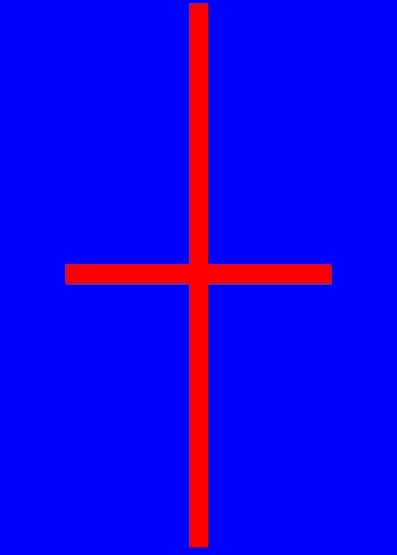
\includegraphics[width=0.3\textwidth]{znacznik.jpg}
	\caption{Wybrana postać znacznika}
	\label{fig:znacznik}
\end{figure}




\section{Analiza kąta widzenia kamery przy różnych ustawieniach rozdzielczości}
\label{sec:wyznaczenie_kata_widzenia_kamery_przy_roznych_ustawieniach}
W~celu zbadania kąta widzenia kamery stworzono moduł nakładający na~obraz prostopadłe linie przecinające się w~jego środku. 
Następnie umieszczono kamerę na wysokości 49 cm i~skierowano ją w~dół. 
Odczytanie odległości od~środka obrazu do~jego krawędzi w~poziomie i~pionie pozwoliło na wyznaczenie kątów widzenia kamery. 
Skorzystano ze wzoru \eqref{eq:kat}.
\begin{equation}
\label{eq:kat}
\alpha=2\arctan{\frac{l}{h}}
\end{equation}
gdzie:
\begin{eqwhere}[2cm]
	\item[$\alpha$] kąt widzenia kamery,
	\item[$h$] wysokość, na jakiej umieszczona jest kamera,
	\item[$l$] odległość środka obrazu od jego krawędzi.
\end{eqwhere}
Na podstawie obrazu przedstawionego na rysunku \ref{fig:1080p} obliczono kąty widzenia kamery w~pionie i~poziomie dla rozdzielczości 1920 x 1080. 
Dla rozdzielczości 1280 x 720 skorzystano z~obrazu pokazanego na rysunku \ref{fig:720p}. 
Korzystając ze wzoru \eqref{eq:kat} otrzymano przybliżone wyniki, przedstawione w tabeli \ref{tab:rozdzielczosc}.
\begin{table}[]
	\caption{Wartości kąta widzenia kamery w zależności od rozdzielczości}
	\label{tab:rozdzielczosc}
	\centering
	\begin{tabular}{|c|c|c|}
		\hline
		\begin{tabular}[c]{@{}c@{}}Rozdzielczość\end{tabular} &  Kąt widzenia kamery w pionie &  Kąt widzenia kamery w poziomie  \\ \hline
		1920 x 1080                                                                          & 28\degree & 54\degree \\ \hline
		1280 x 720                                                                         & 38\degree & 76\degree \\ \hline
	\end{tabular}
\end{table}

\begin{figure}
	\centering
	\begin{subfigure}{0.7\textwidth}
		\centering
		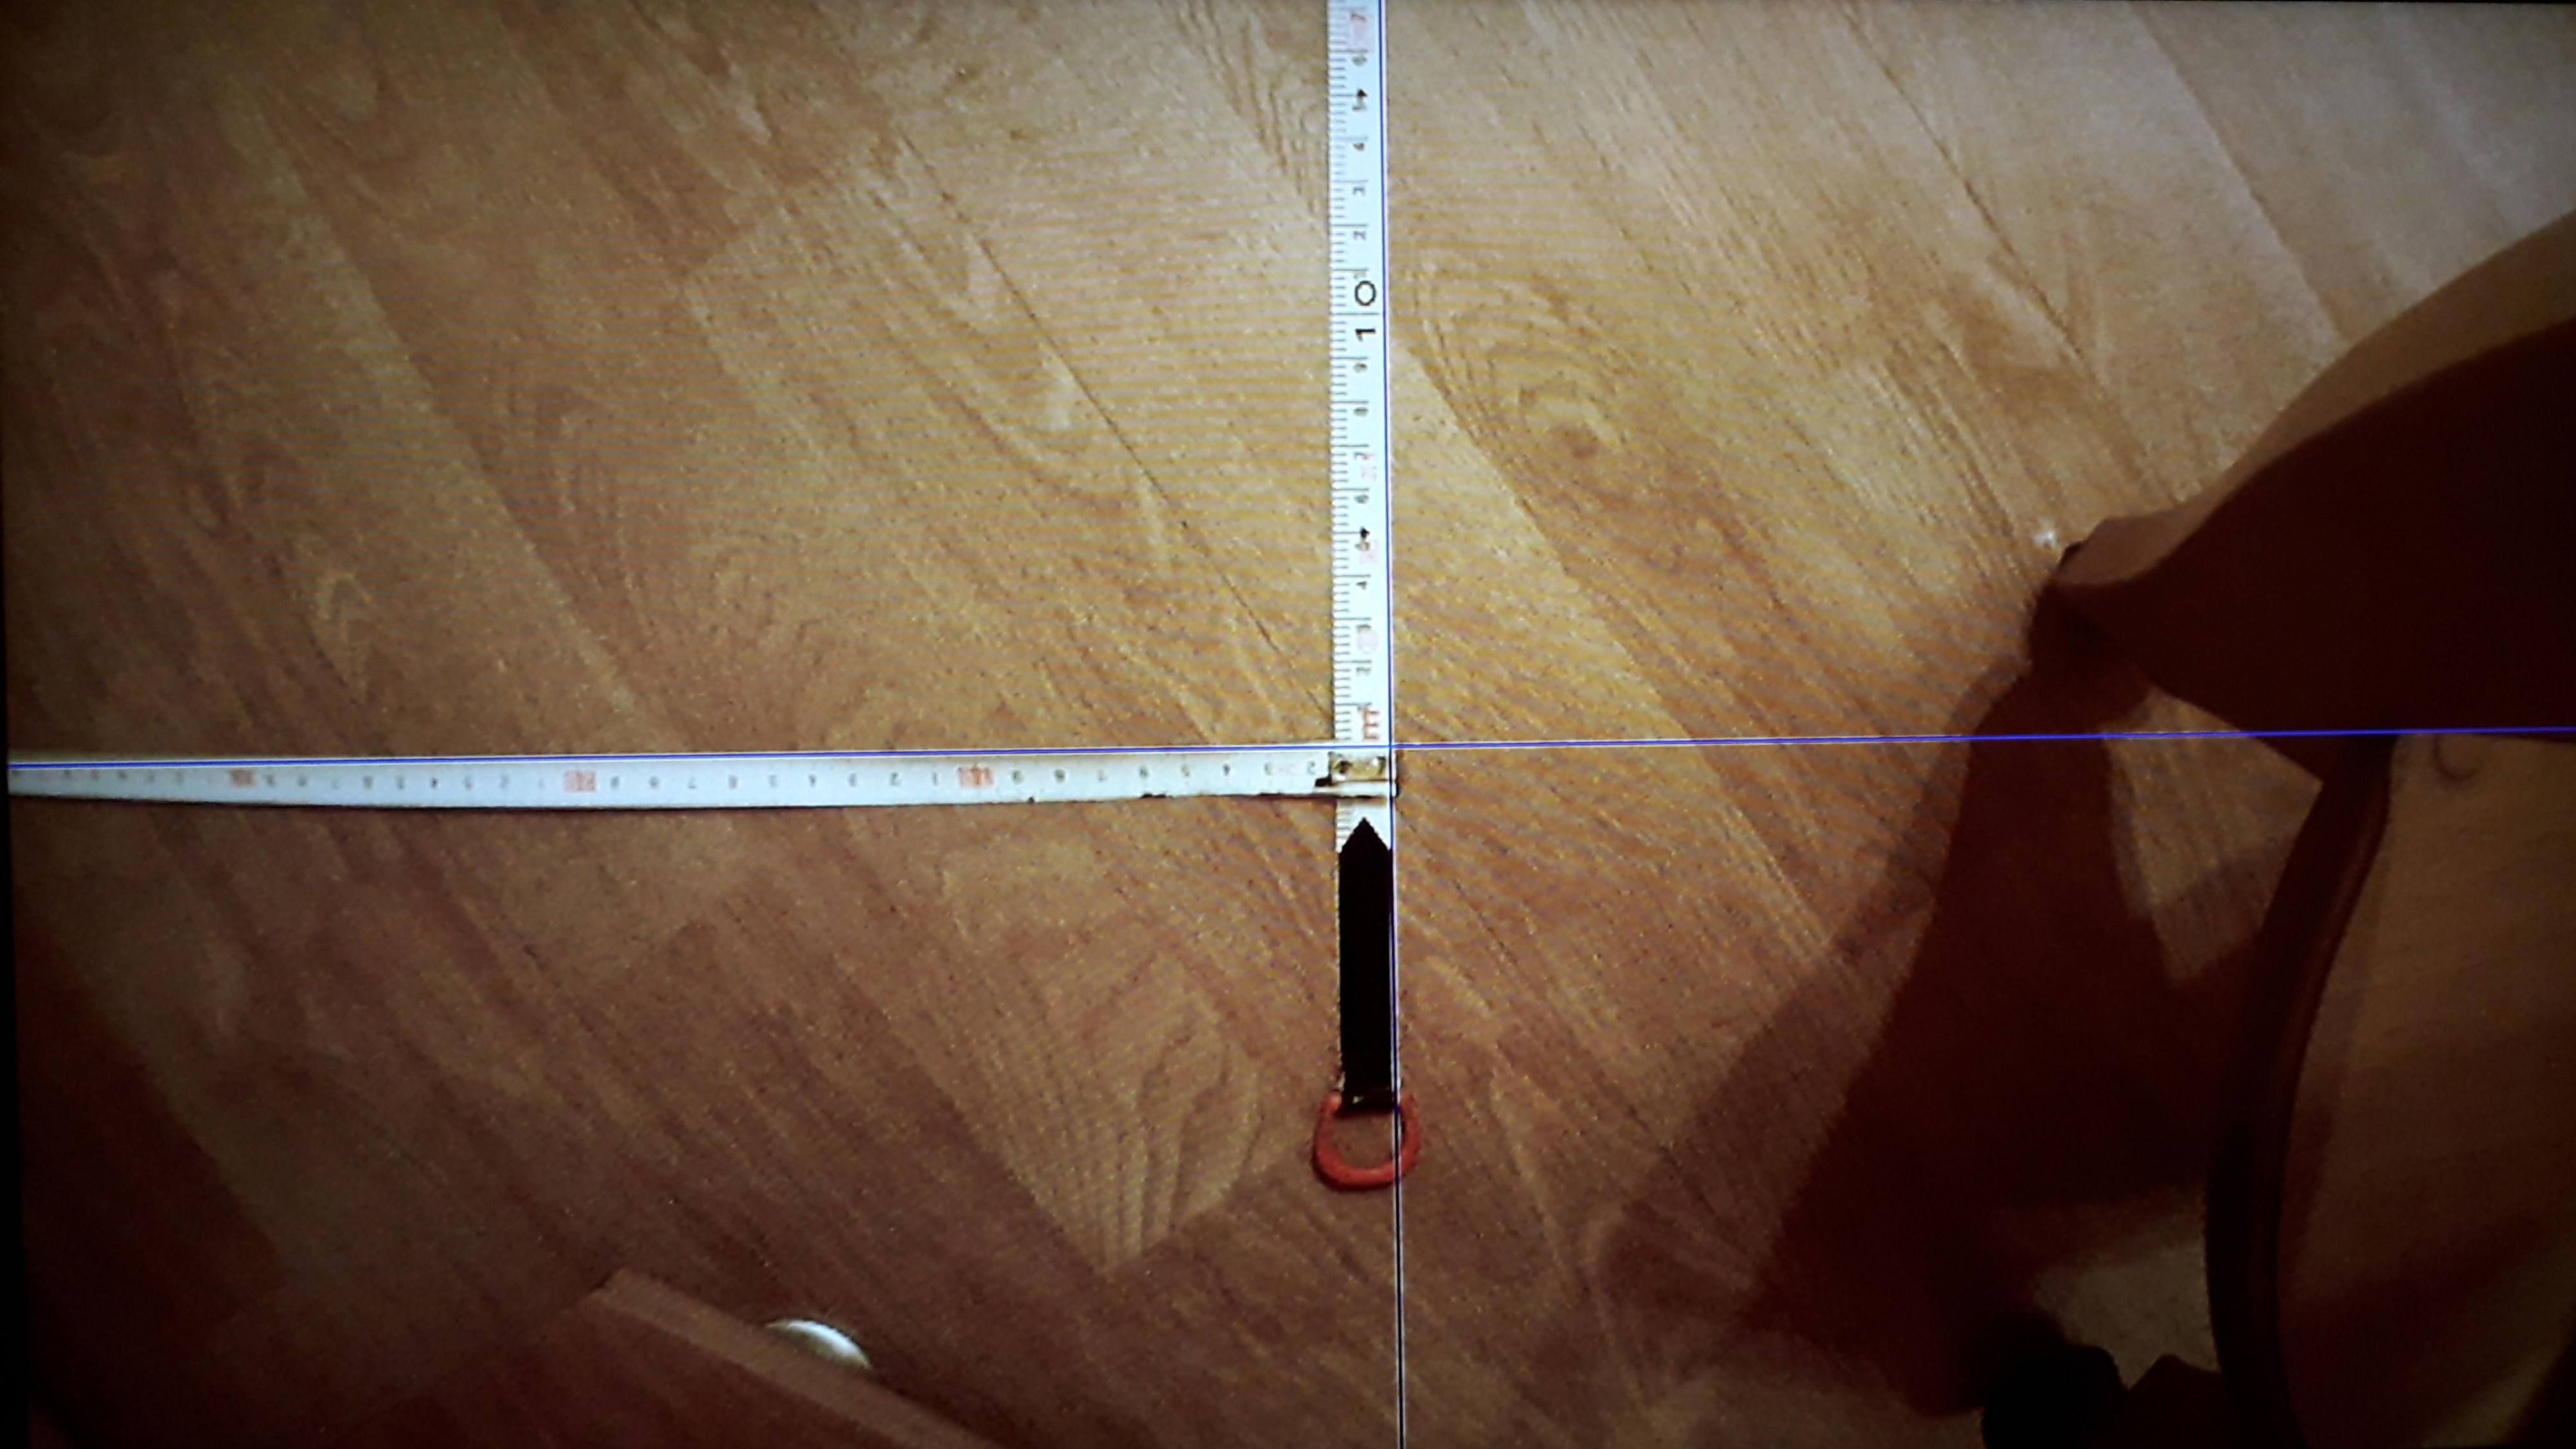
\includegraphics[width=0.9\textwidth]{720p.jpg}
		\caption{Rozdzielczość 1280 x 720.}
		\label{fig:1080p}
	\end{subfigure}
	\begin{subfigure}{0.7\textwidth}
		\centering
		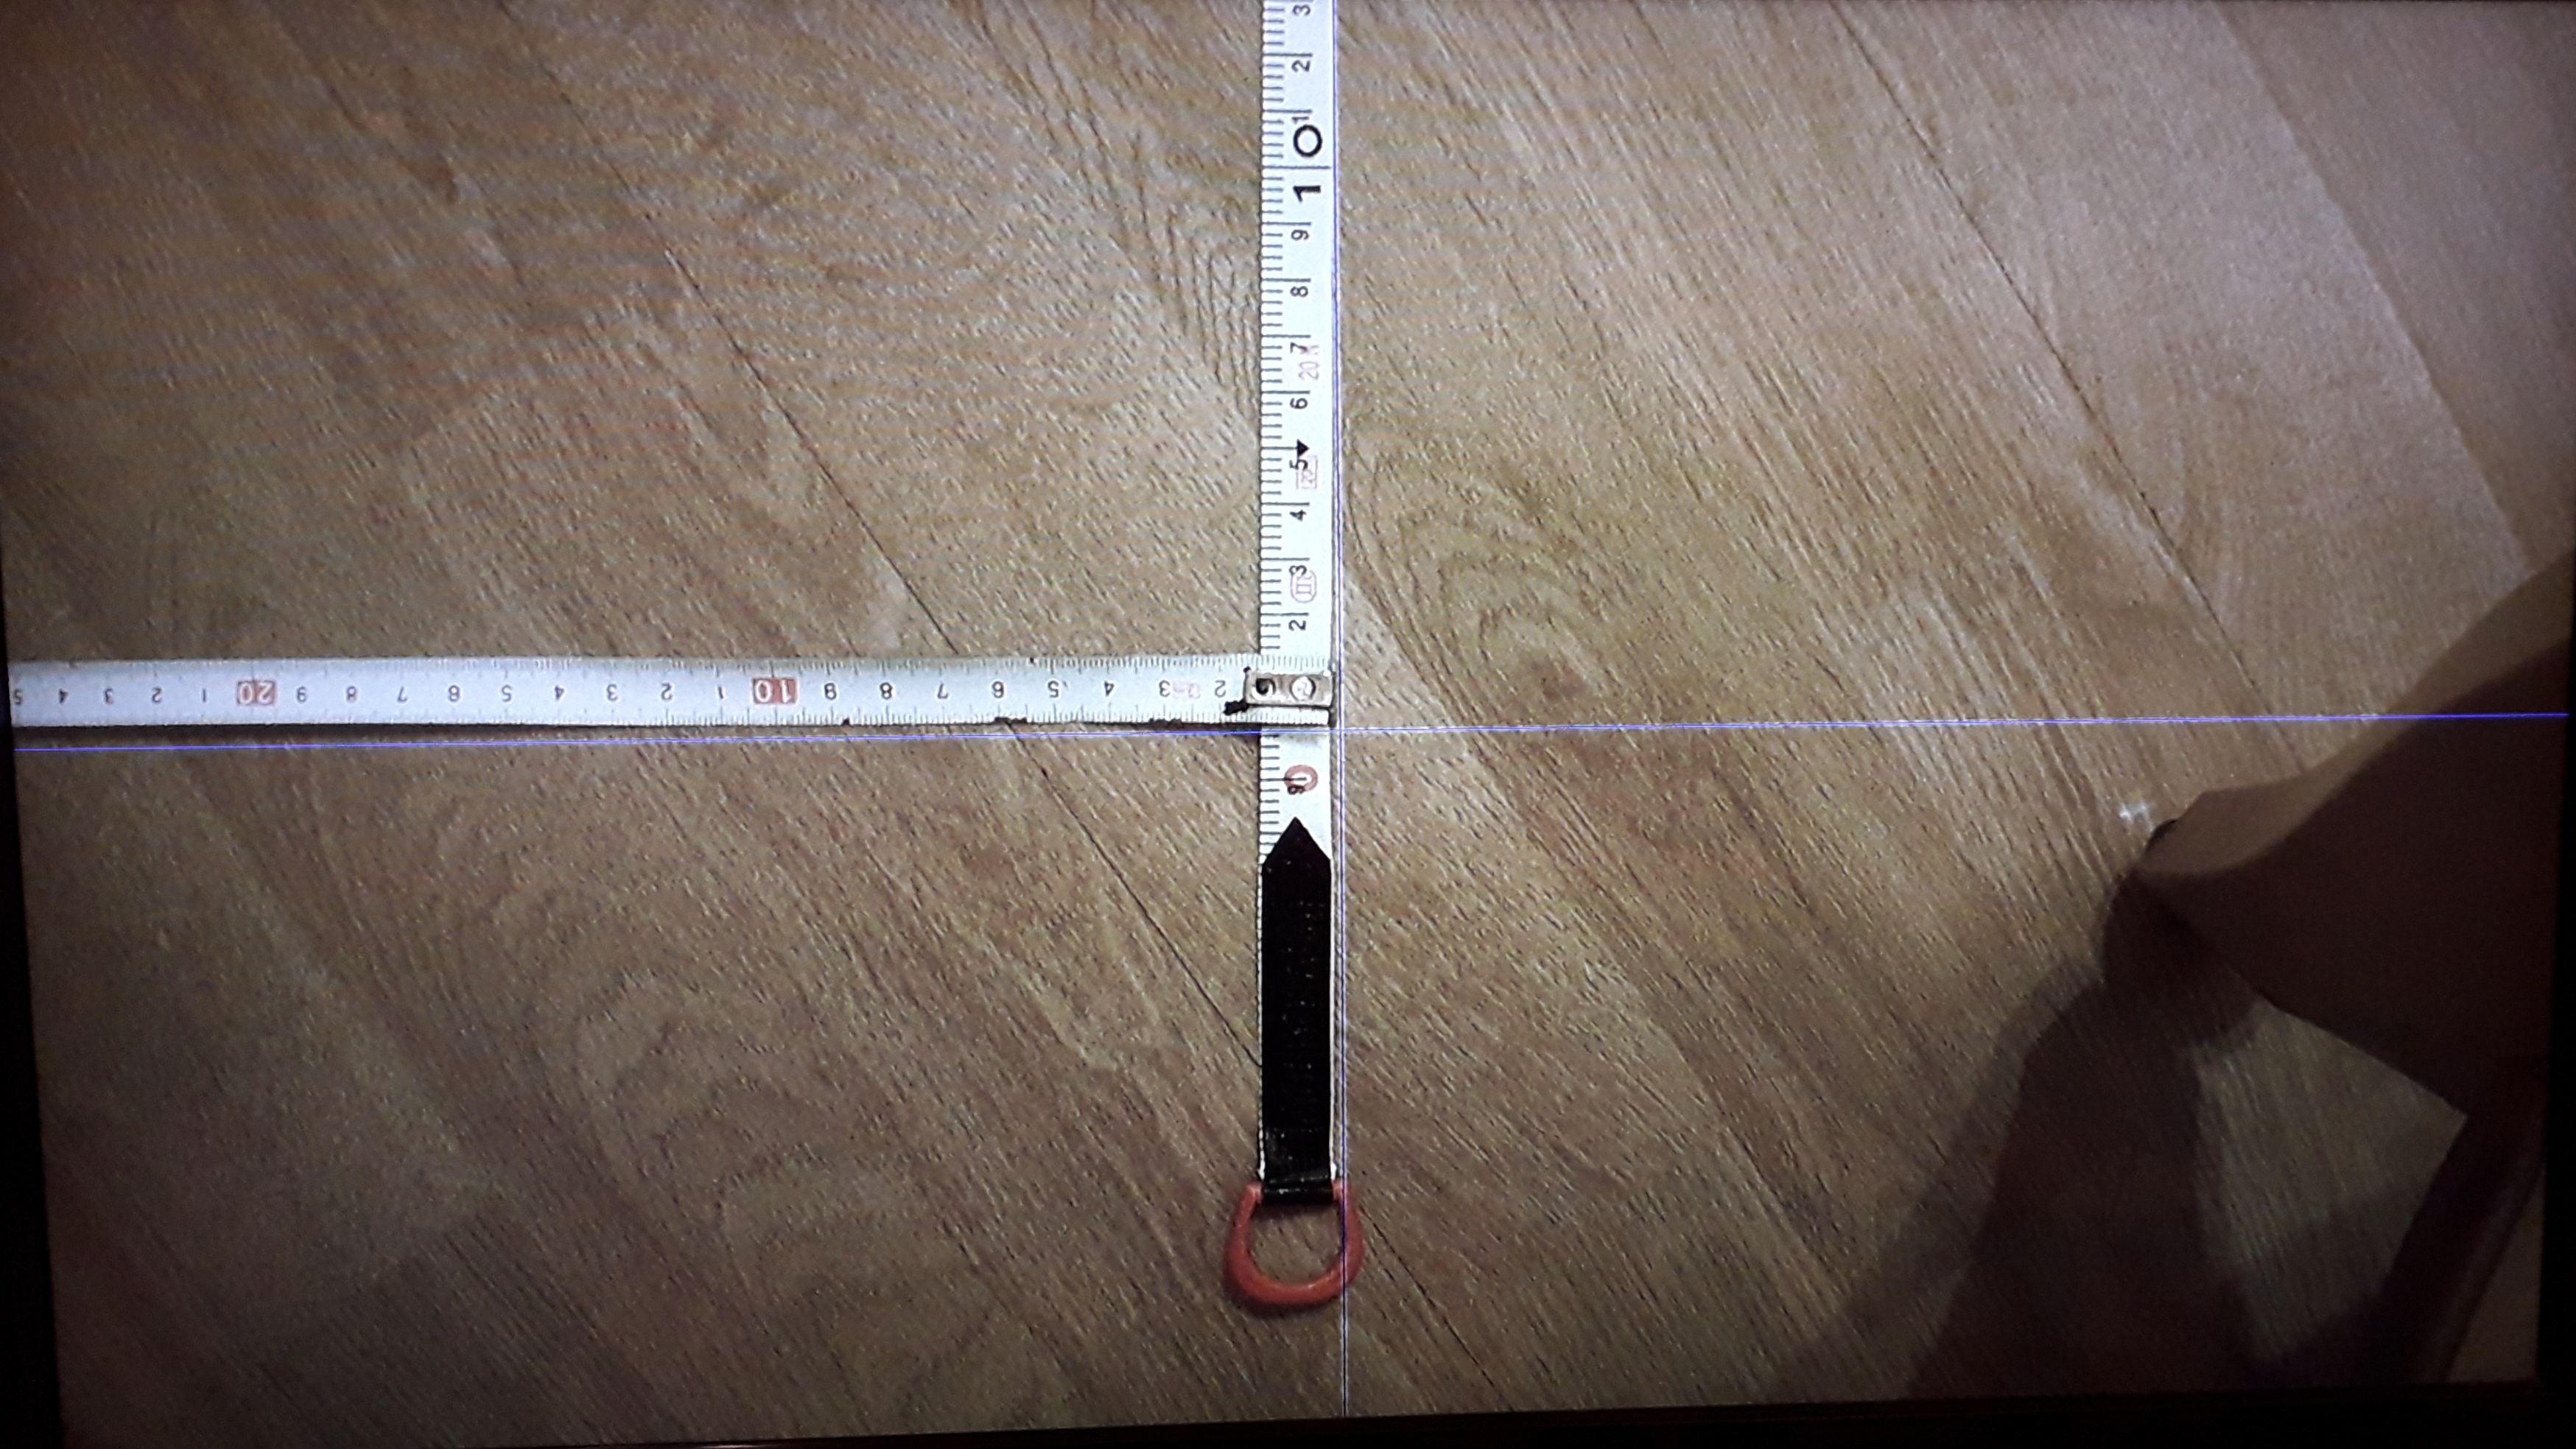
\includegraphics[width=0.9\textwidth]{1080p.jpg}
		\caption{Rozdzielczość 1920 x 1080.}
		\label{fig:720p}
	\end{subfigure}
	\caption{Obrazy służące do wyznaczenia kąta widzenia kamery.}
	\label{fig:rozdzielczosc}
\end{figure}

Tak jak napisano w~podrozdziale \ref{sec:akwizycja}, dla rozdzielczości 1280~x~720 kąt widzenia kamery jest większy, co w~połączeniu z~mniejszą liczbą pikseli do~przetworzenia zdecydowało o~wyborze tej rozdzielczości.
Uzyskane wyniki oznaczają również, że~z~wysokości 1~m dron byłby w~stanie wykryć obiekty w~odległości 34~cm z~przodu i~z~tyłu, oraz 78~cm po~bokach.

\section{Podsumowanie}


Implementacja modelu programowego umożliwiła przetestowanie działania poszczególnych modułów przetwarzania wizyjnego. 
Narzędzia programu Matlab okazały się również bardzo pomocne w~analizie koloru znacznika. 
Sprawdzenie kąta widzenia kamery pozwoliło zorientować się z~jakiej odległości lądowisko będzie dla drona widoczne.




